\documentclass[11pt,letterpaper]{article}
\usepackage[margin=1in]{geometry}
\usepackage[T1]{fontenc}
\usepackage[utf8]{inputenc}
\usepackage{lmodern}
\usepackage{amsmath,amssymb}
\usepackage{array,longtable}
\usepackage{xcolor}
\usepackage{listings}
\usepackage{seqsplit}
\usepackage{graphicx}
\usepackage{float}
\usepackage{microtype}
\usepackage[hidelinks]{hyperref}
\setlength{\parindent}{0pt}
\setlength{\parskip}{6pt}
\setlength{\emergencystretch}{3em}
\lstset{basicstyle=\ttfamily\scriptsize,breaklines=true,
  breakatwhitespace=false,columns=fullflexible,keepspaces=true,
  showstringspaces=false,frame=single,rulecolor=\color{gray!40},
  commentstyle=\color{black!60},tabsize=4}
\title{Programmable Birdsong Synthesizer\\\large ECE 4760: Laboratory 1}
\author{[GROUP MEMBERS AND NETIDS]}
\date{[SUBMISSION DATE]}
\begin{document}
\maketitle
% Upload this file and the figures folder into Overleaf.
% Scope captures and spectrograms remain placeholders, not fabricated results.



ECE 4760: Laboratory 1\\
Authors: [GROUP MEMBERS AND NETIDS]\\
Laboratory dates: [DATES]\\
Source reviewed: September 20, 2026

\textbf{Draft status.} This report documents the saved implementation and the milestones the group reports completing. Numerical values identified as nominal or calculated come from source inspection, not laboratory measurements. Replace bracketed fields and insert the required experimental figures before submission. The demonstrated firmware version and physical wiring must be confirmed by the group.

\section*{1. Introduction}

We developed a programmable tone and birdsong synthesizer using a Raspberry Pi Pico 2 build configuration, a slide potentiometer, a matrix keypad, and an SPI digital-to-analog converter. The potentiometer controls a sinusoidal tone over a nominal 0--10 kHz range. The keypad provides muting, storage of nine frequency trajectories, accelerated playback, and entry of a composition whose elements are the stored sounds. A sound can be previewed while entering a composition, making the interface behave like a soundboard.

The project separates audio generation from user interaction. A timer interrupt generates successive waveform samples using direct digital synthesis (DDS), while cooperative protothreads read the controls, record frequencies, manage playback, and change amplitude. Recording the frequency trajectory rather than the audio waveform lets a small memory buffer represent several seconds of sound. Reading that trajectory ten times faster produces rapid frequency modulation without multiplying the carrier frequency.

The assignment is the ECE 4760 version of \href{https://vanhunteradams.com/Pico/Birds/Birdsong.html}{Synthesizing Birdsong with the RP2350}. Its checkpoints progress from DAC and ADC integration to recording and accelerated composition. The additional ECE 5730 volume-switch extension is outside this report's scope.

\section*{2. Design and Testing Methods}

\subsection*{2.1 Incremental development and milestone mapping}

The repository preserves separate programs for successive stages. These are implementation evidence, rather than independent proof of a successful hardware checkout. The group reports meeting the milestones; checkout dates and observations should be added below.

\begingroup\small
\setlength{\tabcolsep}{5pt}
\begin{longtable}{|>{\raggedright\arraybackslash}p{0.295\linewidth}|>{\raggedright\arraybackslash}p{0.295\linewidth}|>{\raggedright\arraybackslash}p{0.295\linewidth}|}
\hline
\textbf{Checkpoint} & \textbf{Repository evidence} & \textbf{Verification or remaining evidence} \\ \hline
\endhead
Preparation: build course examples & Pico SDK import and CMake project & Confirm initial successful build and programming procedure \\ \hline
Week 1: fixed tone and DAC output & \texttt{dactest.c}: 800 Hz DDS command, channel A & Scope waveform and audible output; measured frequency [ ] \\ \hline
Week 1: change DAC channel & \texttt{dactest\_other\_channel.c}: channel B control word & Probe B and confirm output moved; observation [ ] \\ \hline
Week 1: external boot button & Build links \texttt{pico\_bootsel\_via\_double\_reset} & This library does not prove the external button was wired; add circuit/photo and checkout result \\ \hline
Week 1: potentiometer and ADC & \texttt{ADC\_with\_DDS.c}: ADC channel 0 mapped to 0--10,000 Hz & Endpoint/intermediate ADC and frequency measurements [ ] \\ \hline
Week 2: keypad integration and mute & \texttt{ADC\_DDS\_keypad\_mute.c}: four-state debounce and amplitude ramp & Repeated press/hold/release test; result [ ] \\ \hline
Week 2: nine recordings and normal-speed playback & \texttt{ADC\_DDS\_keypad\_record.c}: frequency buffers and 10 ms playback & Distinct recordings, replacement, hold/release behavior; result [ ] \\ \hline
Week 2: interrupt timing & GPIO 2 surrounds synthesis ISR & High-pulse width and period [ ] \\ \hline
Week 3: live tone at boot and return via 0 & \texttt{ADC\_DDS\_keypad\_speedup.c}: initial tone enabled; mode cancellation on 0 & Startup and mode-transition tests [ ] \\ \hline
Week 3: accelerated playback & Final file: 10 ms record, 1 ms playback & Nominal 10:1; measured duration ratio [ ] \\ \hline
Week 3: composition and sound previews & Final file: nine-entry sequence; indirect lookup of stored sound & Nonconsecutive/repeated-key sequence and interrupted-preview test [ ] \\ \hline
Week 3: demonstration without restart & Final state transitions support repeated operation & Group/TA observation, cardinal imitation, and Merlin result [ ] \\ \hline
\end{longtable}
\endgroup

Historical programs explain development; only \texttt{ADC\_DDS\_keypad\_speedup.c} is selected by the current CMake target. No claim is made that every historical file represents the exact version demonstrated.

\subsection*{2.2 Hardware approach}

The source configures SPI0 for 16-bit transfers at a requested 20 MHz, with clock polarity and phase both zero. The final program sends the channel-A configuration word followed by a 12-bit DAC code in the same 16-bit frame. The assignment specifies an MCP4822 DAC; the actual installed component should be confirmed against the breadboard. The command uses unity gain and enables the selected channel.

The slide potentiometer wiper connects to GPIO 26, which is ADC input 0. Its endpoints should connect to the analog supply range and ground so that the wiper remains within the ADC input range. Four keypad rows use GPIO 9--12, and three columns use GPIO 13--15 with internal pull-ups. Each scan drives one row low, waits 1 microsecond, and reads the columns. The code compares the resulting pattern against a lookup table to identify digits, asterisk, and hash.

The functional block diagram and pin-assignment table give a logical interconnect derived from the program. They are not a substitute for the as-built schematic: DAC latch wiring, supply bypassing, external boot circuitry, audio-jack connections, and any coupling components must be added from the actual setup.

The hardware photographs document two stages of assembly. The initial setup shows the controller, DAC circuit, audio socket, and oscilloscope probing. The later setup includes the slide potentiometer and telephone-style keypad. The photographs establish the physical arrangement but do not resolve every electrical connection.

\begin{figure}[H]
\centering
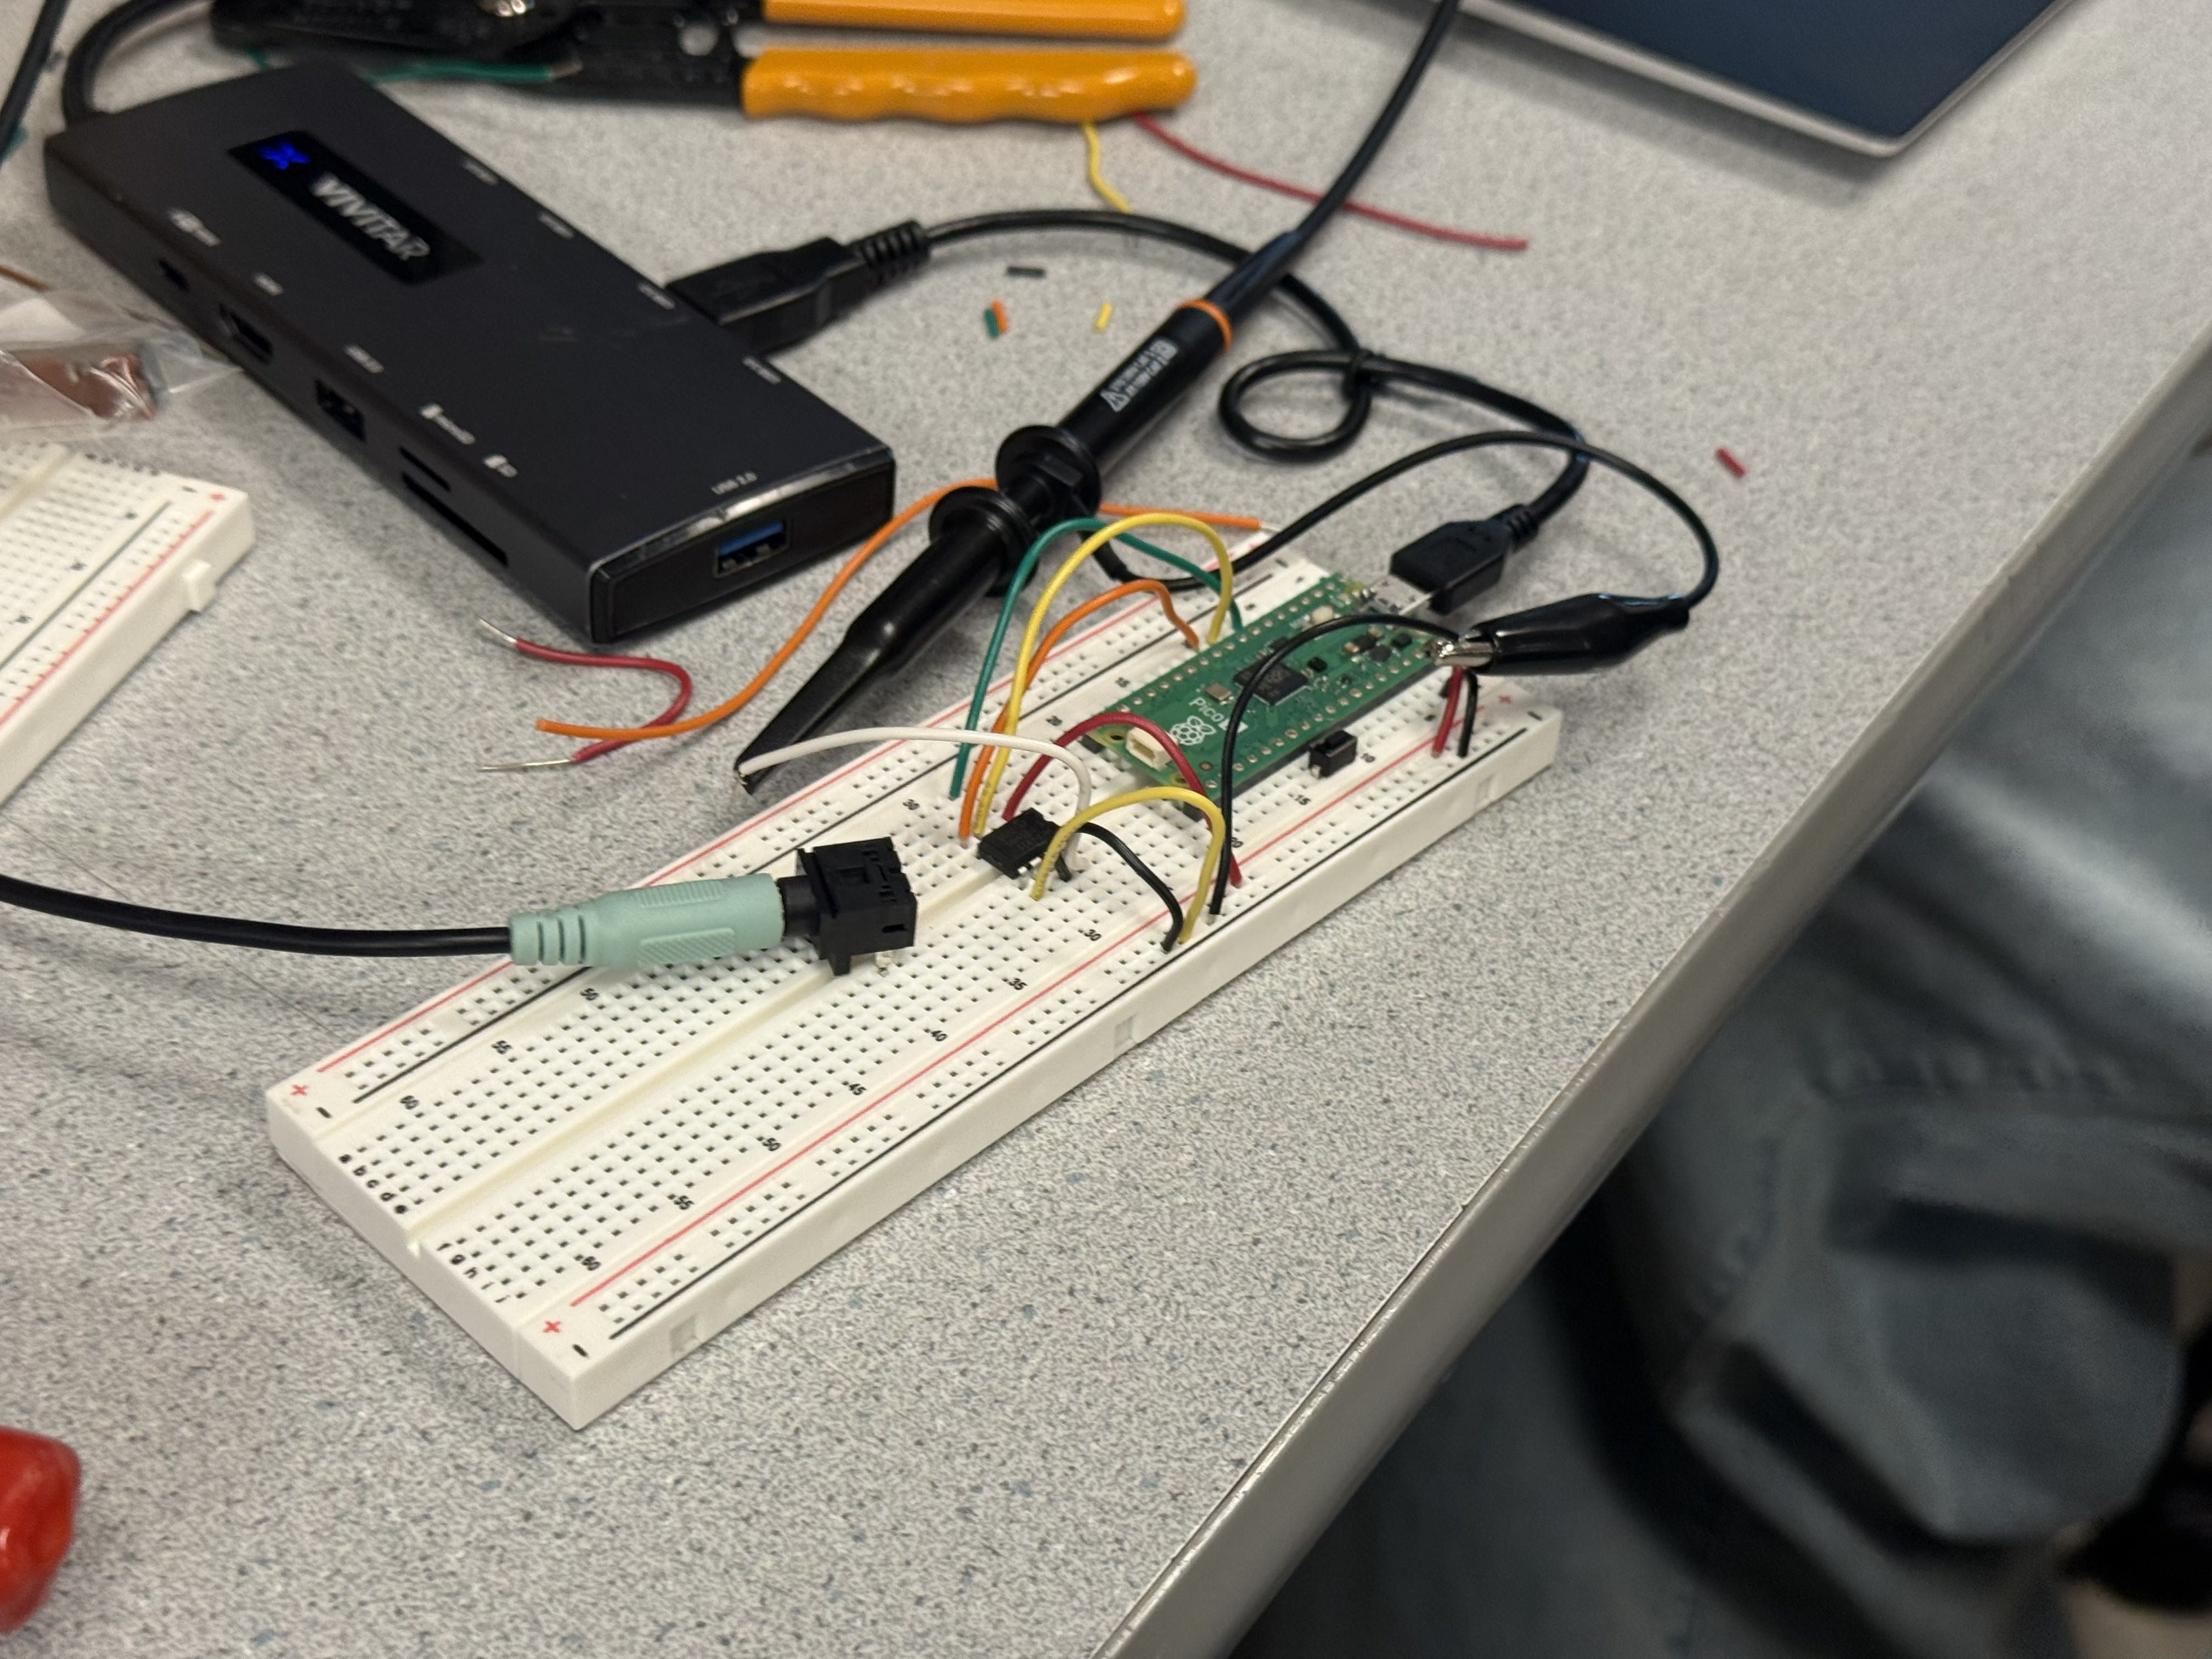
\includegraphics[width=\linewidth,height=0.65\textheight,keepaspectratio]{figures/dac_breadboard.jpg}
\caption{Initial DAC and audio-output breadboard setup, including the controller, audio socket, USB connection, and oscilloscope probes. Photograph: IMG\_7768.}
\end{figure}

\begin{figure}[H]
\centering
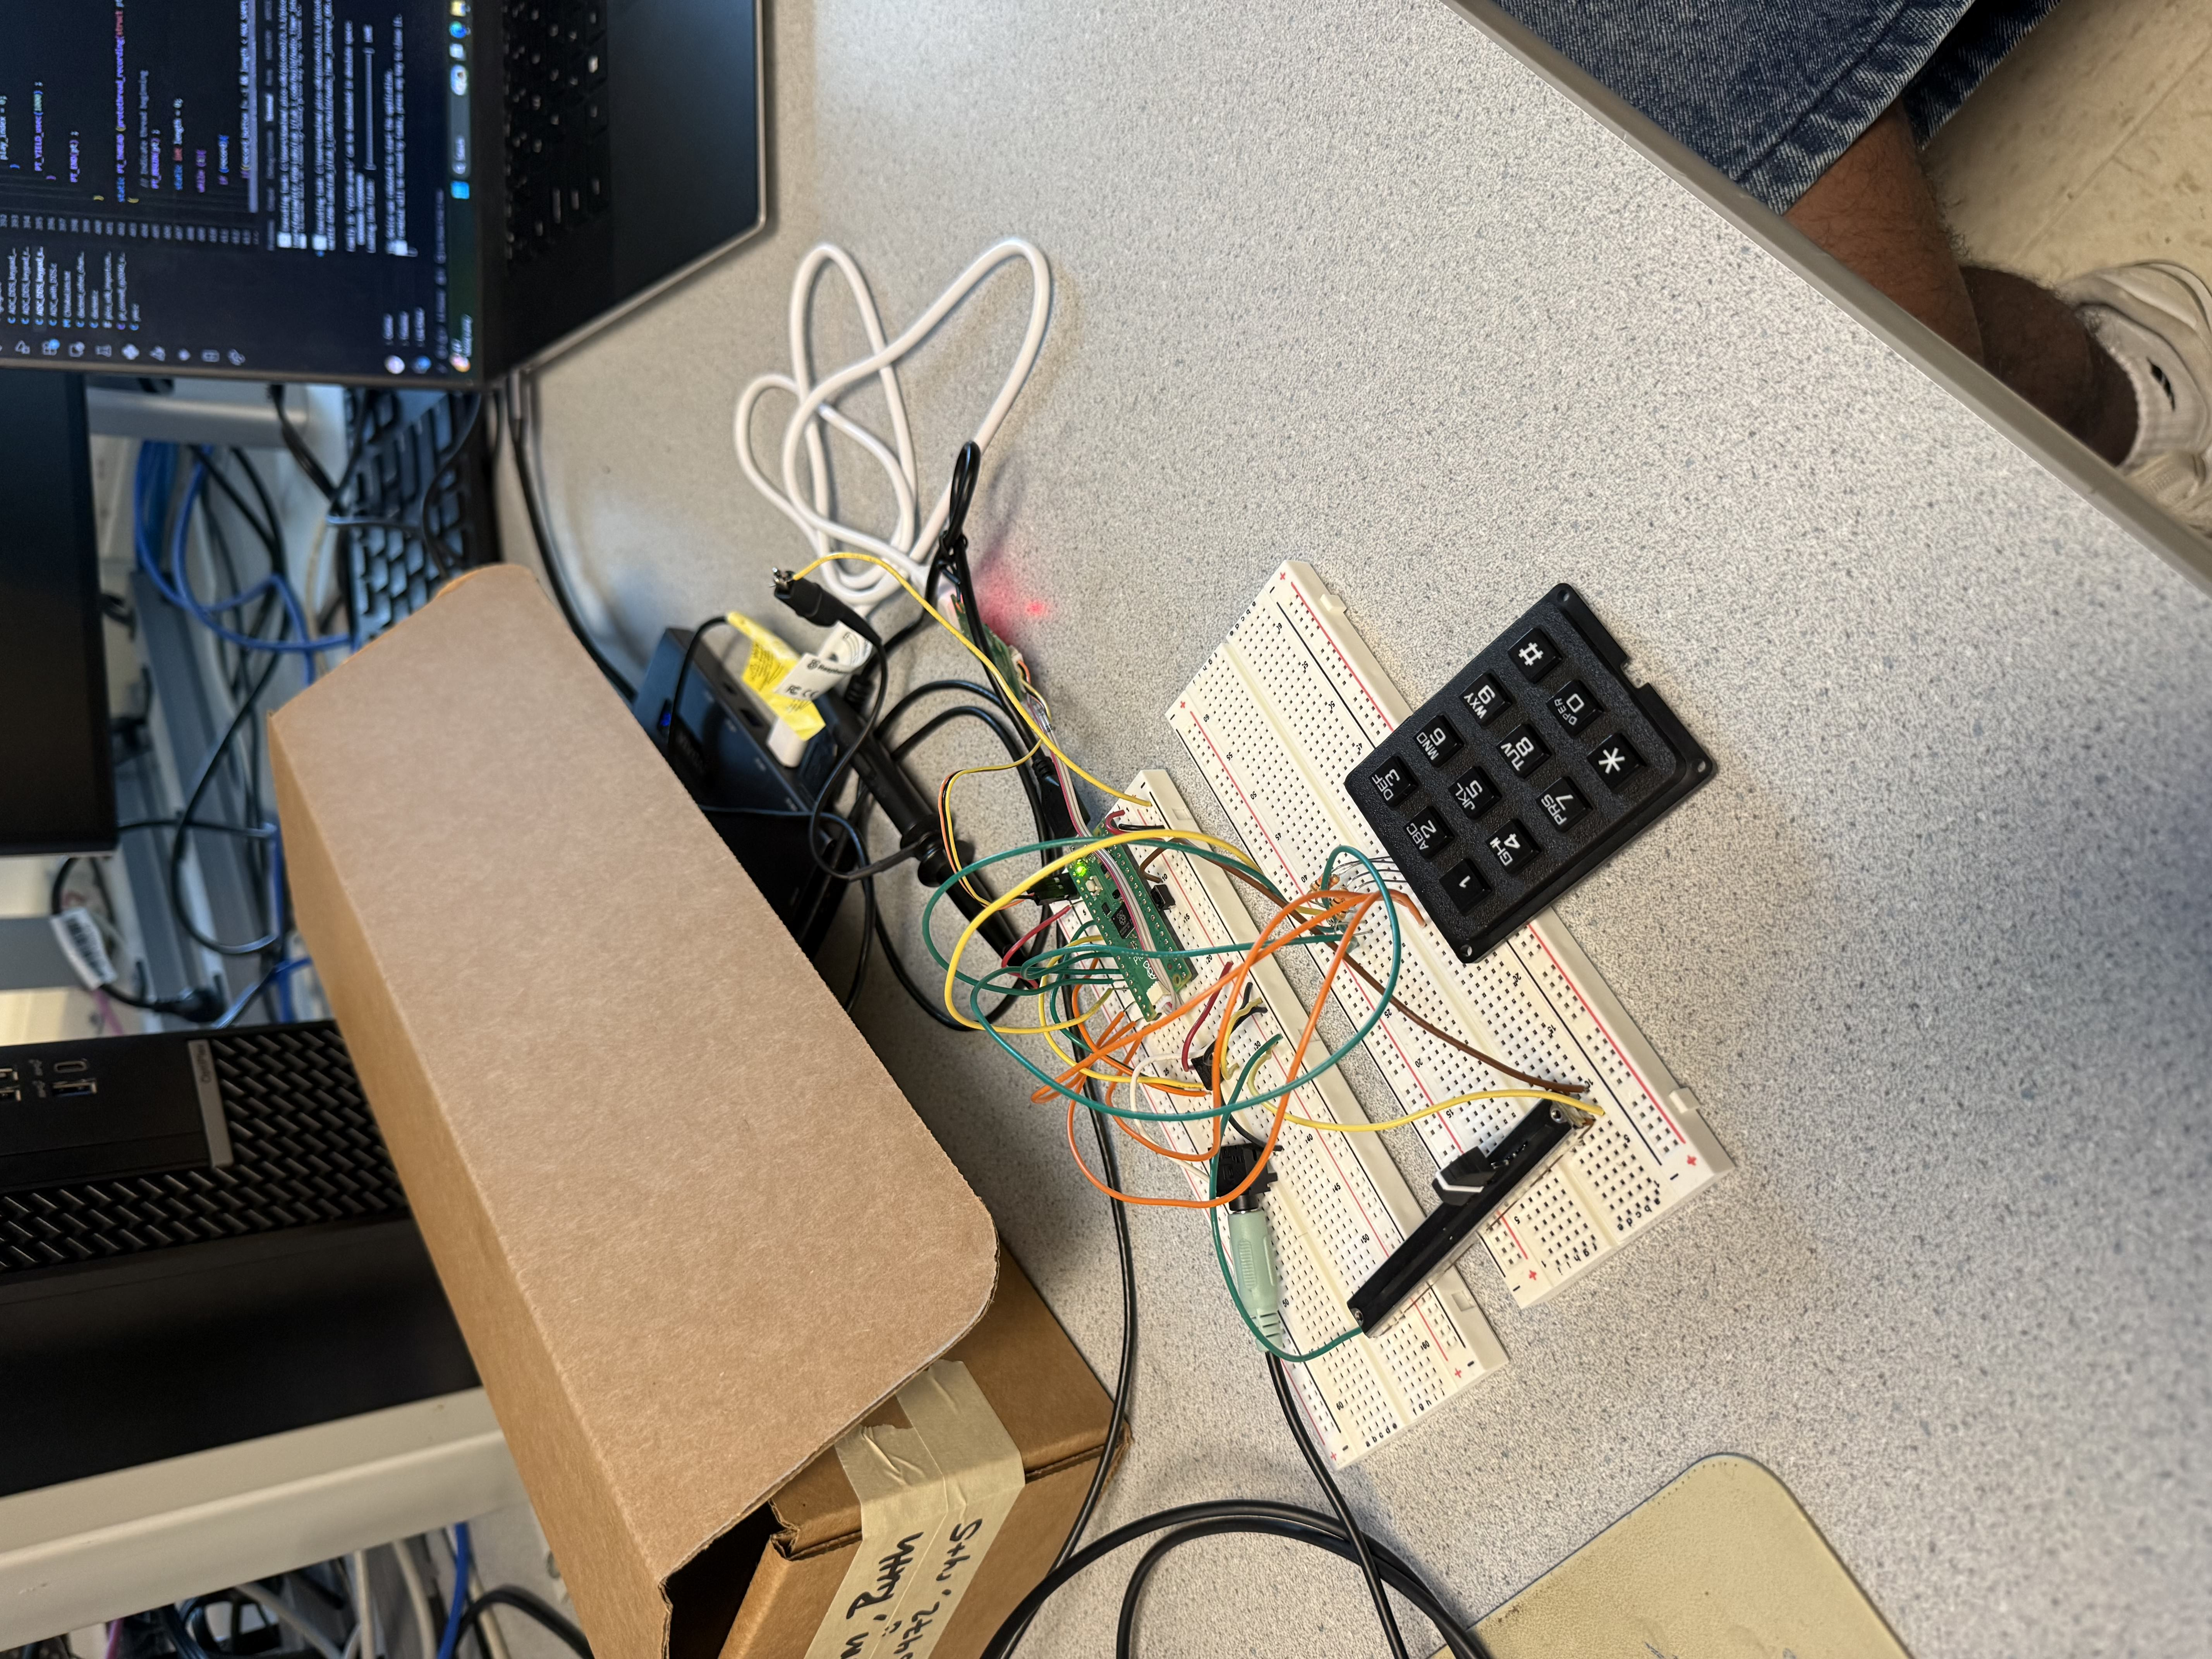
\includegraphics[angle=-90,width=\linewidth,height=0.65\textheight,keepaspectratio]{figures/keypad_potentiometer_setup.jpg}
\caption{Integrated synthesizer setup with the slide potentiometer, matrix keypad, controller, and audio-output wiring. Photograph: IMG\_7908.}
\end{figure}

\subsection*{2.3 DDS and amplitude control}

For ADC code a, the requested frequency is calculated using integer arithmetic:

\texttt{f\_command = floor(a \ensuremath{\times} 10000 / 4095)} Hz.

The requested phase increment is:

\texttt{\ensuremath{\Delta} = floor(f\_command \ensuremath{\times} 2\textasciicircum{}32 / 50000)}.

At each interrupt, the unsigned 32-bit phase accumulator is advanced by \ensuremath{\Delta}. Overflow naturally wraps the phase. The upper eight bits select one of 256 entries in a sine table initialized with \texttt{2047 \ensuremath{\times} sin(2\ensuremath{\pi}i/256)}; the source uses 6.283 as its approximation to 2\ensuremath{\pi}. A signed sample is scaled by the amplitude variable before adding a midpoint offset:

\texttt{DAC\_code = 2048 + trunc(sine\_table[phase >> 24] \ensuremath{\times} amplitude / 2047)}.

The normal bounds are 1--4095 at full amplitude, with silence represented by a constant midpoint code of 2048. Muting therefore removes the AC waveform; it does not drive the DAC output to zero volts. The phase accumulator keeps advancing while muted.

Amplitude is clamped between 0 and 2047. The final amplitude thread changes it by 103 and yields for 50 microseconds. A full transition needs 20 updates, giving an approximate 1 ms ramp timescale before scheduling delays. The comment describing 1 ms updates is stale; the earlier mute version did use that slower interval. This envelope applies to playback start/stop transitions, not automatically to every individual element inside a composition.

\subsection*{2.4 Recording, playback, and concurrency}

Five protothreads run on the default core scheduler. Although multicore, DMA, and PIO headers are included, the final application does not launch a second core or use DMA/PIO for synthesis.

\begingroup\small
\setlength{\tabcolsep}{5pt}
\begin{longtable}{|>{\raggedright\arraybackslash}p{0.295\linewidth}|>{\raggedright\arraybackslash}p{0.295\linewidth}|>{\raggedright\arraybackslash}p{0.295\linewidth}|}
\hline
\textbf{Routine} & \textbf{Role} & \textbf{Requested yield} \\ \hline
\endhead
\texttt{protothread\_toggle25} & Read ADC, print commanded frequency, update live-tone increment when playback is inactive & 10 ms \\ \hline
\texttt{protothread\_core\_0} & Scan keypad, debounce, dispatch mode actions & 30 ms \\ \hline
\texttt{protothread\_amplitude} & Move amplitude toward its enabled/muted target & 50 \ensuremath{\mu}s \\ \hline
\texttt{protothread\_playback} & Select successive frequencies from an individual sound or composition & 1 ms \\ \hline
\texttt{protothread\_recording} & Append frequency values while recording & 10 ms \\ \hline
\texttt{alarm\_irq} & Advance DDS and transfer DAC sample & Nominal 20 \ensuremath{\mu}s alarm interval \\ \hline
\end{longtable}
\endgroup

Recordings use \texttt{uint16\_t sounds[9][1000]} and one valid length per sound. Key k maps to row k\ensuremath{-}1. The sample storage occupies 18,000 bytes and represents nominally ten seconds per key. At 100 Hz, each entry describes the frequency over roughly 10 ms. Playback updates the phase increment every 1 ms, compressing the trajectory to approximately one-tenth its recorded duration. The DAC sample rate remains unchanged, and the stored frequencies are not multiplied by ten.

The recording thread resets its local write index while idle and updates the selected row's length after each write. When the array is full, additional samples are discarded until release. Recordings reside in RAM and are lost on reset or loss of power. A composition stores nine key numbers rather than copying the sound data; consequently, re-recording a key changes the sound referenced by any retained composition.

The live ADC thread yields ownership of \texttt{phase\_incr\_main} whenever either playback flag is set. Mode entry cancels competing playback and resets the sequence and sample positions. Key 0 cancels recording/composition/playback and restores the current potentiometer frequency; if no other mode is active, it toggles the live tone. During compose entry, digit presses both append a key number and preview a nonempty sound. The second hash cancels the preview and begins sequence playback from the first entry.

\subsection*{2.5 Testing methods and acceptance evidence}

The following is the verification procedure for this implementation. The supplied photographs document a sinusoidal output and a timing pulse. Other procedures below remain proposed verification tests unless accompanied by the group's recorded results.

\begin{enumerate}
\item \textbf{DAC and tone calibration.} Run the fixed-tone test on A, then the channel-B variant. Measure frequency, DC midpoint, peak-to-peak amplitude, and waveform shape. In the ADC program, record ADC code and measured frequency at both endpoints and several intermediate positions. At the zero-frequency endpoint, expect a stationary DAC code rather than a periodic waveform.
\item \textbf{Debounce and mode entry.} Hold 0 through several scans and verify exactly one action. Repeat with deliberately slow releases and with asterisk/hash. Observe whether the action occurs on press or release. Verify that the current program acts on confirmed press even though comments describe release.
\item \textbf{Recording isolation.} Store distinguishable sweeps on keys 1, 5, and 9; replay each; overwrite key 5 with a shorter trajectory; confirm the others are unchanged and no old tail remains. Test a long hold at the capacity limit and a very short hold.
\item \textbf{Speed measurement.} Record a trajectory containing identifiable frequency transitions. Measure its recording interval and the corresponding playback interval, then calculate \texttt{S = T\_record / T\_play}. Repeat to estimate variation; compare S with the requested 8--10 range. Keep serial-output conditions the same as during the demonstration.
\item \textbf{Composition.} Enter a nonconsecutive sequence such as 9, 1, 9, 5. Verify each preview and the final ordering. Start sequence playback while a preview is still active. Interrupt the sequence with a soundboard key, then test return via 0 and entry via asterisk/hash without resetting the board. Test empty slots, an empty composition, and a tenth sequence entry.
\item \textbf{Audio quality and timing.} Capture a complete programmed sweep with its amplitude envelope. Measure rise, sustain, and fall times and inspect any discontinuity at sequence boundaries. Probe GPIO 2 for ISR high time and repetition period under normal and heavy keypad/serial activity. Capture audio for a spectrogram and compare the frequency trajectory with the intended birdcall.
\end{enumerate}

For each frequency point, report signed error \texttt{f\_measured \ensuremath{-} f\_command} and percentage error for nonzero commands. Report instrument resolution or cursor uncertainty. For speed ratio uncertainty, independent duration uncertainties can be propagated as \texttt{\ensuremath{\sigma}S/S \ensuremath{\approx} sqrt((\ensuremath{\sigma}Tr/Tr)\textasciicircum{}2 + (\ensuremath{\sigma}Tp/Tp)\textasciicircum{}2)}. Do not assign an error bar solely from software resolution.

\subsection*{2.6 Use of AI}

We used an AI coding assistant through an iterative dialogue to explain DDS amplitude and frequency control, inspect the debounce state machine, compare code with the lab behavior, and suggest implementations for recording and composition. The conversation records advice about missing switch breaks, array bounds and lengths, frequency-versus-phase-increment storage, playback timing, ADC ownership during playback, sequence indexing, and mode reset behavior. The group repeatedly requested reviews without file changes and made subsequent revisions themselves.

One visible assistant edit changed an earlier keypad source to shorten the fade, relocate its toggle to a release transition, register the keypad/amplitude threads, and remove an undefined LED reference. Later revisions do not retain every suggestion: the final source still dispatches control actions on confirmed press. Code visible in the final file supports adoption of several other suggestions, including fixed-size frequency buffers, bounded amplitude updates, sequence indirection, and the key-0 return-to-tone behavior.

AI output was treated as a proposal to inspect, not experimental evidence. No scope timings, spectral measurements, successful identification results, or acceptance statistics were invented. Appendix B records the available provenance and the limitations of reconstructing a complete prompt log. The group must verify this disclosure and supply the full exported dialogue for the required audit.

\section*{3. Documentation}

\subsection*{3.1 Logical wiring and signal flow}

\begin{figure}[H]
\centering
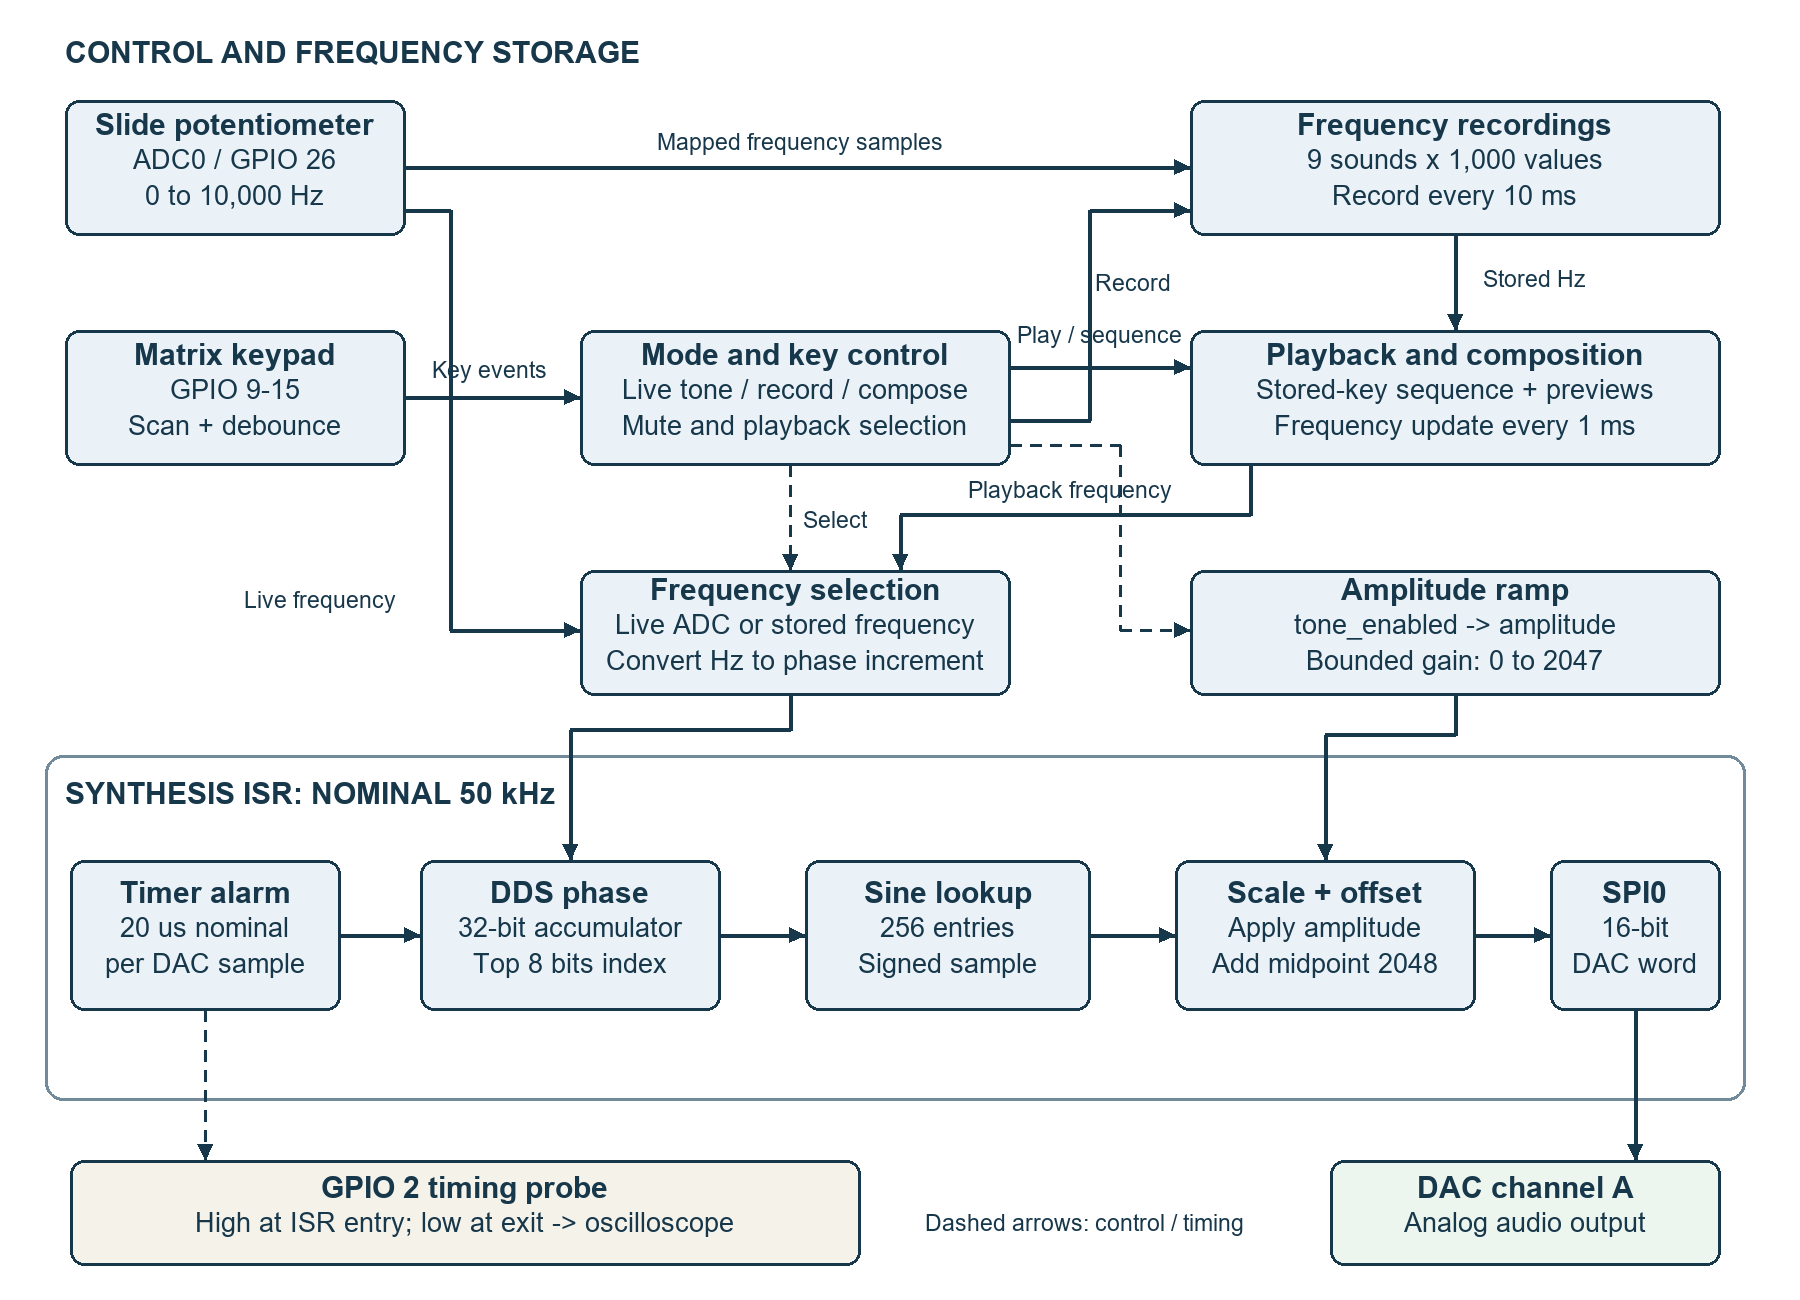
\includegraphics[width=\linewidth,height=0.65\textheight,keepaspectratio]{figures/signal_flow.png}
\caption{Functional signal flow derived from the saved implementation. Dashed arrows indicate control or timing signals; this is not an as-built wiring schematic.}
\end{figure}

\begingroup\small
\setlength{\tabcolsep}{5pt}
\begin{longtable}{|>{\raggedright\arraybackslash}p{0.295\linewidth}|>{\raggedright\arraybackslash}p{0.295\linewidth}|>{\raggedright\arraybackslash}p{0.295\linewidth}|}
\hline
\textbf{Pico signal} & \textbf{Program assignment} & \textbf{External connection / confirmation} \\ \hline
\endhead
GPIO 5 & SPI0 chip select & DAC active-low CS \\ \hline
GPIO 6 & SPI0 clock & DAC SCK \\ \hline
GPIO 7 & SPI0 transmit & DAC SDI \\ \hline
GPIO 4 & SPI0 receive function configured & No DAC read transaction is used \\ \hline
GPIO 26 & ADC0 & Potentiometer wiper \\ \hline
GPIO 9--12 & Row outputs & Keypad rows; confirm connector order \\ \hline
GPIO 13--15 & Pulled-up column inputs & Keypad columns; confirm connector order \\ \hline
GPIO 2 & ISR timing output & Scope probe \\ \hline
GPIO 25 & LED toggle output & Code assignment; board-specific LED behavior is not verification of audio \\ \hline
Supply and ground & Not established by C source & Add actual DAC, potentiometer, and shared-ground wiring \\ \hline
DAC latch, audio socket, boot button & Not established by C source & Add actual connections and any component values \\ \hline
\end{longtable}
\endgroup

\begin{figure}[H]
\centering
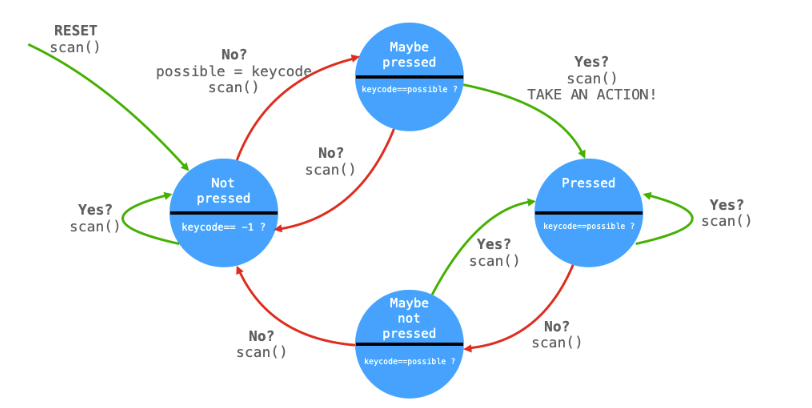
\includegraphics[width=\linewidth,height=0.65\textheight,keepaspectratio]{figures/debounce_state_machine.png}
\caption{Four-state keypad debounce diagram supplied by the group. The action on confirmed press matches the saved implementation; recording ends on confirmed release.}
\end{figure}

Because the keypad thread yields between scans and every switch case ends with a break, a single observation cannot pass through all debounce states. The remembered key identifies the recording to stop after the raw input no longer names that key. A different valid key is treated as loss of the previous key; this is a single-key interface, not a general multi-key rollover implementation.

\subsection*{3.2 Reproduction and program listings}

The current build selects \texttt{ADC\_DDS\_keypad\_speedup.c} in target \texttt{Audio\_Timer\_Interrupt\_DDS}, with \texttt{PICO\_BOARD} set to \texttt{pico2}. The CMake configuration names SDK 2.3.0 and toolchain 15\_2\_Rel1 and includes the local \texttt{pt\_cornell\_rp2040\_v1\_4.h}. Reproduction requires the SDK import file, the matching SDK/toolchain setup, the protothreads header, and the selected application source. Configure and build using the Pico extension or the existing CMake workflow, then program the generated UF2 using the board's bootloader procedure. Confirm the actual board and tool versions used during checkout.

Appendix A is a complete, source-preserving listing of all six C files and CMake configuration, with explanatory annotations added only to the documentation. It includes an inventory and hashes so later code changes can be distinguished from this report's snapshot. The application files were not edited to prepare this report.

\section*{4. Results}

\subsection*{4.1 Source-derived performance}

\begingroup\small
\setlength{\tabcolsep}{5pt}
\begin{longtable}{|>{\raggedright\arraybackslash}p{0.295\linewidth}|>{\raggedright\arraybackslash}p{0.295\linewidth}|>{\raggedright\arraybackslash}p{0.295\linewidth}|}
\hline
\textbf{Quantity} & \textbf{Calculated or configured value} & \textbf{Interpretation} \\ \hline
\endhead
Audio sample rate & 50,000 samples/s nominal & Set by 20 \ensuremath{\mu}s alarm delay; actual period needs measurement \\ \hline
Frequency command range & 0--10,000 Hz & Integer mapping from ADC code \\ \hline
Mean frequency-command spacing & 10,000/4095 \ensuremath{\approx} 2.442 Hz per ADC code & Actual adjacent integer commands differ by 2 or 3 Hz \\ \hline
DDS increment resolution & 50,000/2\textasciicircum{}32 \ensuremath{\approx} 0.00001164 Hz & Ideal digital tuning granularity, not measured accuracy \\ \hline
Sine table & 256 entries & Phase index resolution 1.40625\ensuremath{^{\circ}} \\ \hline
Record interval & 10 ms nominal & Approximately 100 frequency entries/s \\ \hline
Playback interval & 1 ms nominal & Approximately 10\ensuremath{\times} trajectory speed \\ \hline
Per-key recording limit & 1,000 entries & Approximately 10 s recorded / 1 s accelerated \\ \hline
Frequency storage & 18,000 bytes & Nine arrays of 1,000 unsigned 16-bit values \\ \hline
Composition capacity & Nine entries & Repetitions allowed; no entry timestamps stored \\ \hline
Fade timescale & Approximately 1 ms & 20 updates with 50 \ensuremath{\mu}s yields; timing varies \\ \hline
SPI frame wire time & 16 / 20 MHz = 0.8 \ensuremath{\mu}s nominal & Excludes software and interrupt overhead \\ \hline
\end{longtable}
\endgroup

The interrupt rearms the alarm relative to the timer value read inside the ISR. Interrupt-entry and pre-rearm latency therefore contribute to the effective sample period. DDS uses the nominal 50 kHz constant, so any measured sample-rate error proportionally changes the generated frequency. Similarly, thread yields specify waiting intervals, not guaranteed sampling deadlines. The enabled frequency printout can add scheduling delay. These effects prevent claiming exact 10\ensuremath{\times} speed or exact pitch from source alone.

\subsection*{4.2 Experimental observations and remaining measurements}

\begingroup\small
\setlength{\tabcolsep}{5pt}
\begin{longtable}{|>{\raggedright\arraybackslash}p{0.295\linewidth}|>{\raggedright\arraybackslash}p{0.295\linewidth}|>{\raggedright\arraybackslash}p{0.295\linewidth}|}
\hline
\textbf{Measurement} & \textbf{Observed value} & \textbf{Uncertainty / evidence} \\ \hline
\endhead
Fixed-tone waveform & Scope displays 800.000 Hz & IMG\_7767; DAC output channel and instrument uncertainty not documented \\ \hline
Potentiometer minimum/maximum frequency & [MEASURE] & [ADC codes and scope resolution] \\ \hline
Largest frequency error over tested points & [MEASURE] & [Number/range of points] \\ \hline
Timing-pulse high interval & Cursor separation 1.63 \ensuremath{\mu}s & IMG\_7909; one capture, not a worst-case timing bound \\ \hline
Timing-trace repetition & Scope displays 50.0000 kHz, corresponding to 20.0 \ensuremath{\mu}s & IMG\_7909; period inferred from displayed frequency \\ \hline
Record/playback duration ratio & [MEASURE] & [Repeated trials and variation] \\ \hline
Envelope rise / sustain / fall & [MEASURE] & [Scope figure] \\ \hline
Debounce reliability and mode cycling & [OBSERVATION] & [Test count and failures] \\ \hline
Cardinal imitation / Merlin outcome & [OBSERVATION] & [Spectrogram and demo notes] \\ \hline
\end{longtable}
\endgroup

The fixed-tone photograph shows a sinusoidal waveform with an 800.000 Hz frequency readout. The displayed scales are 500 mV/division and 400 \ensuremath{\mu}s/division. This is consistent with the 800 Hz baseline program. The photo does not establish which DAC output was probed, and the readout precision is not an uncertainty estimate or proof of zero frequency error.

\begin{figure}[H]
\centering
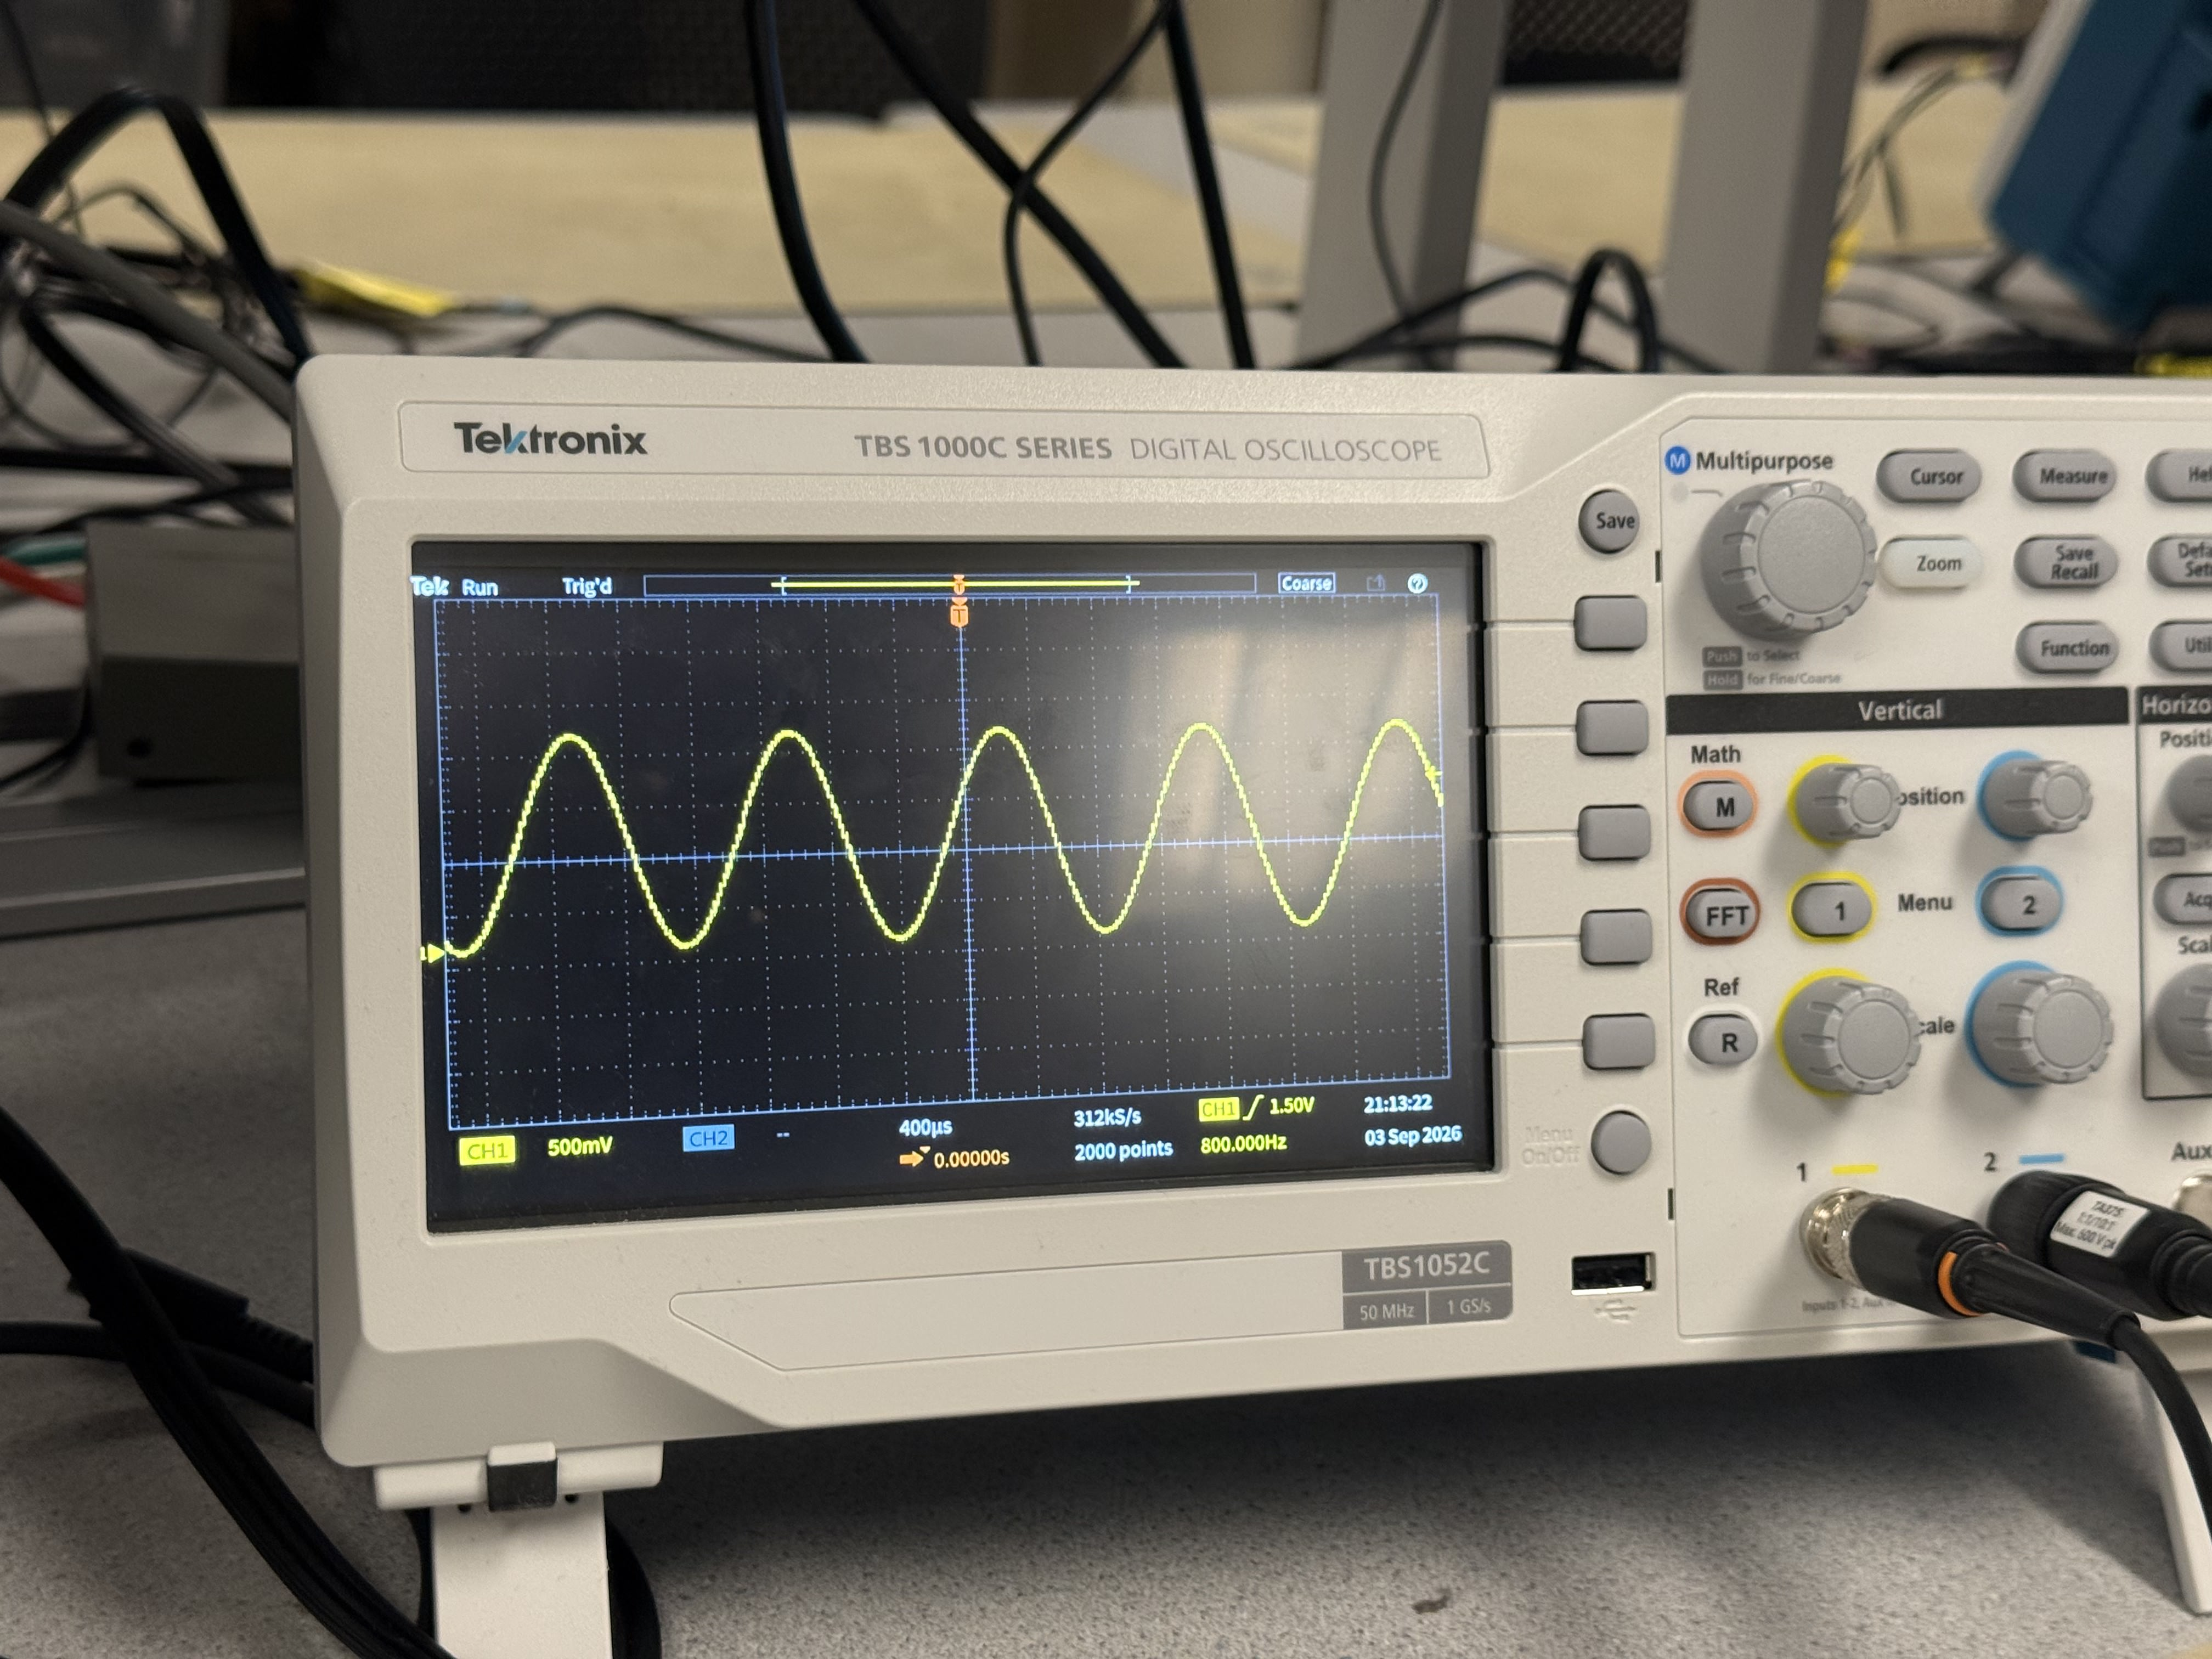
\includegraphics[width=\linewidth,height=0.65\textheight,keepaspectratio]{figures/tone_800hz.jpg}
\caption{Fixed-tone oscilloscope observation: sinusoidal output with an 800.000 Hz readout, 500 mV/division vertical scale, and 400 \ensuremath{\mu}s/division horizontal scale. Photograph: IMG\_7767.}
\end{figure}

The timing photograph shows a high pulse bounded by cursors at approximately -48.0 ns and 1.58 \ensuremath{\mu}s; the instrument reports a 1.63 \ensuremath{\mu}s separation. The displayed frequency is 50.0000 kHz. Interpreting this as the GPIO 2 ISR instrumentation gives an instrumented-body occupancy of approximately 1.63/20.0 = 8.15\%. This interpretation is consistent with the timing code, but the photograph alone does not identify the probe connection or firmware version. The observation is a single captured interval, not a measured maximum across operating conditions. Interrupt overhead outside the GPIO writes is excluded.

\begin{figure}[H]
\centering
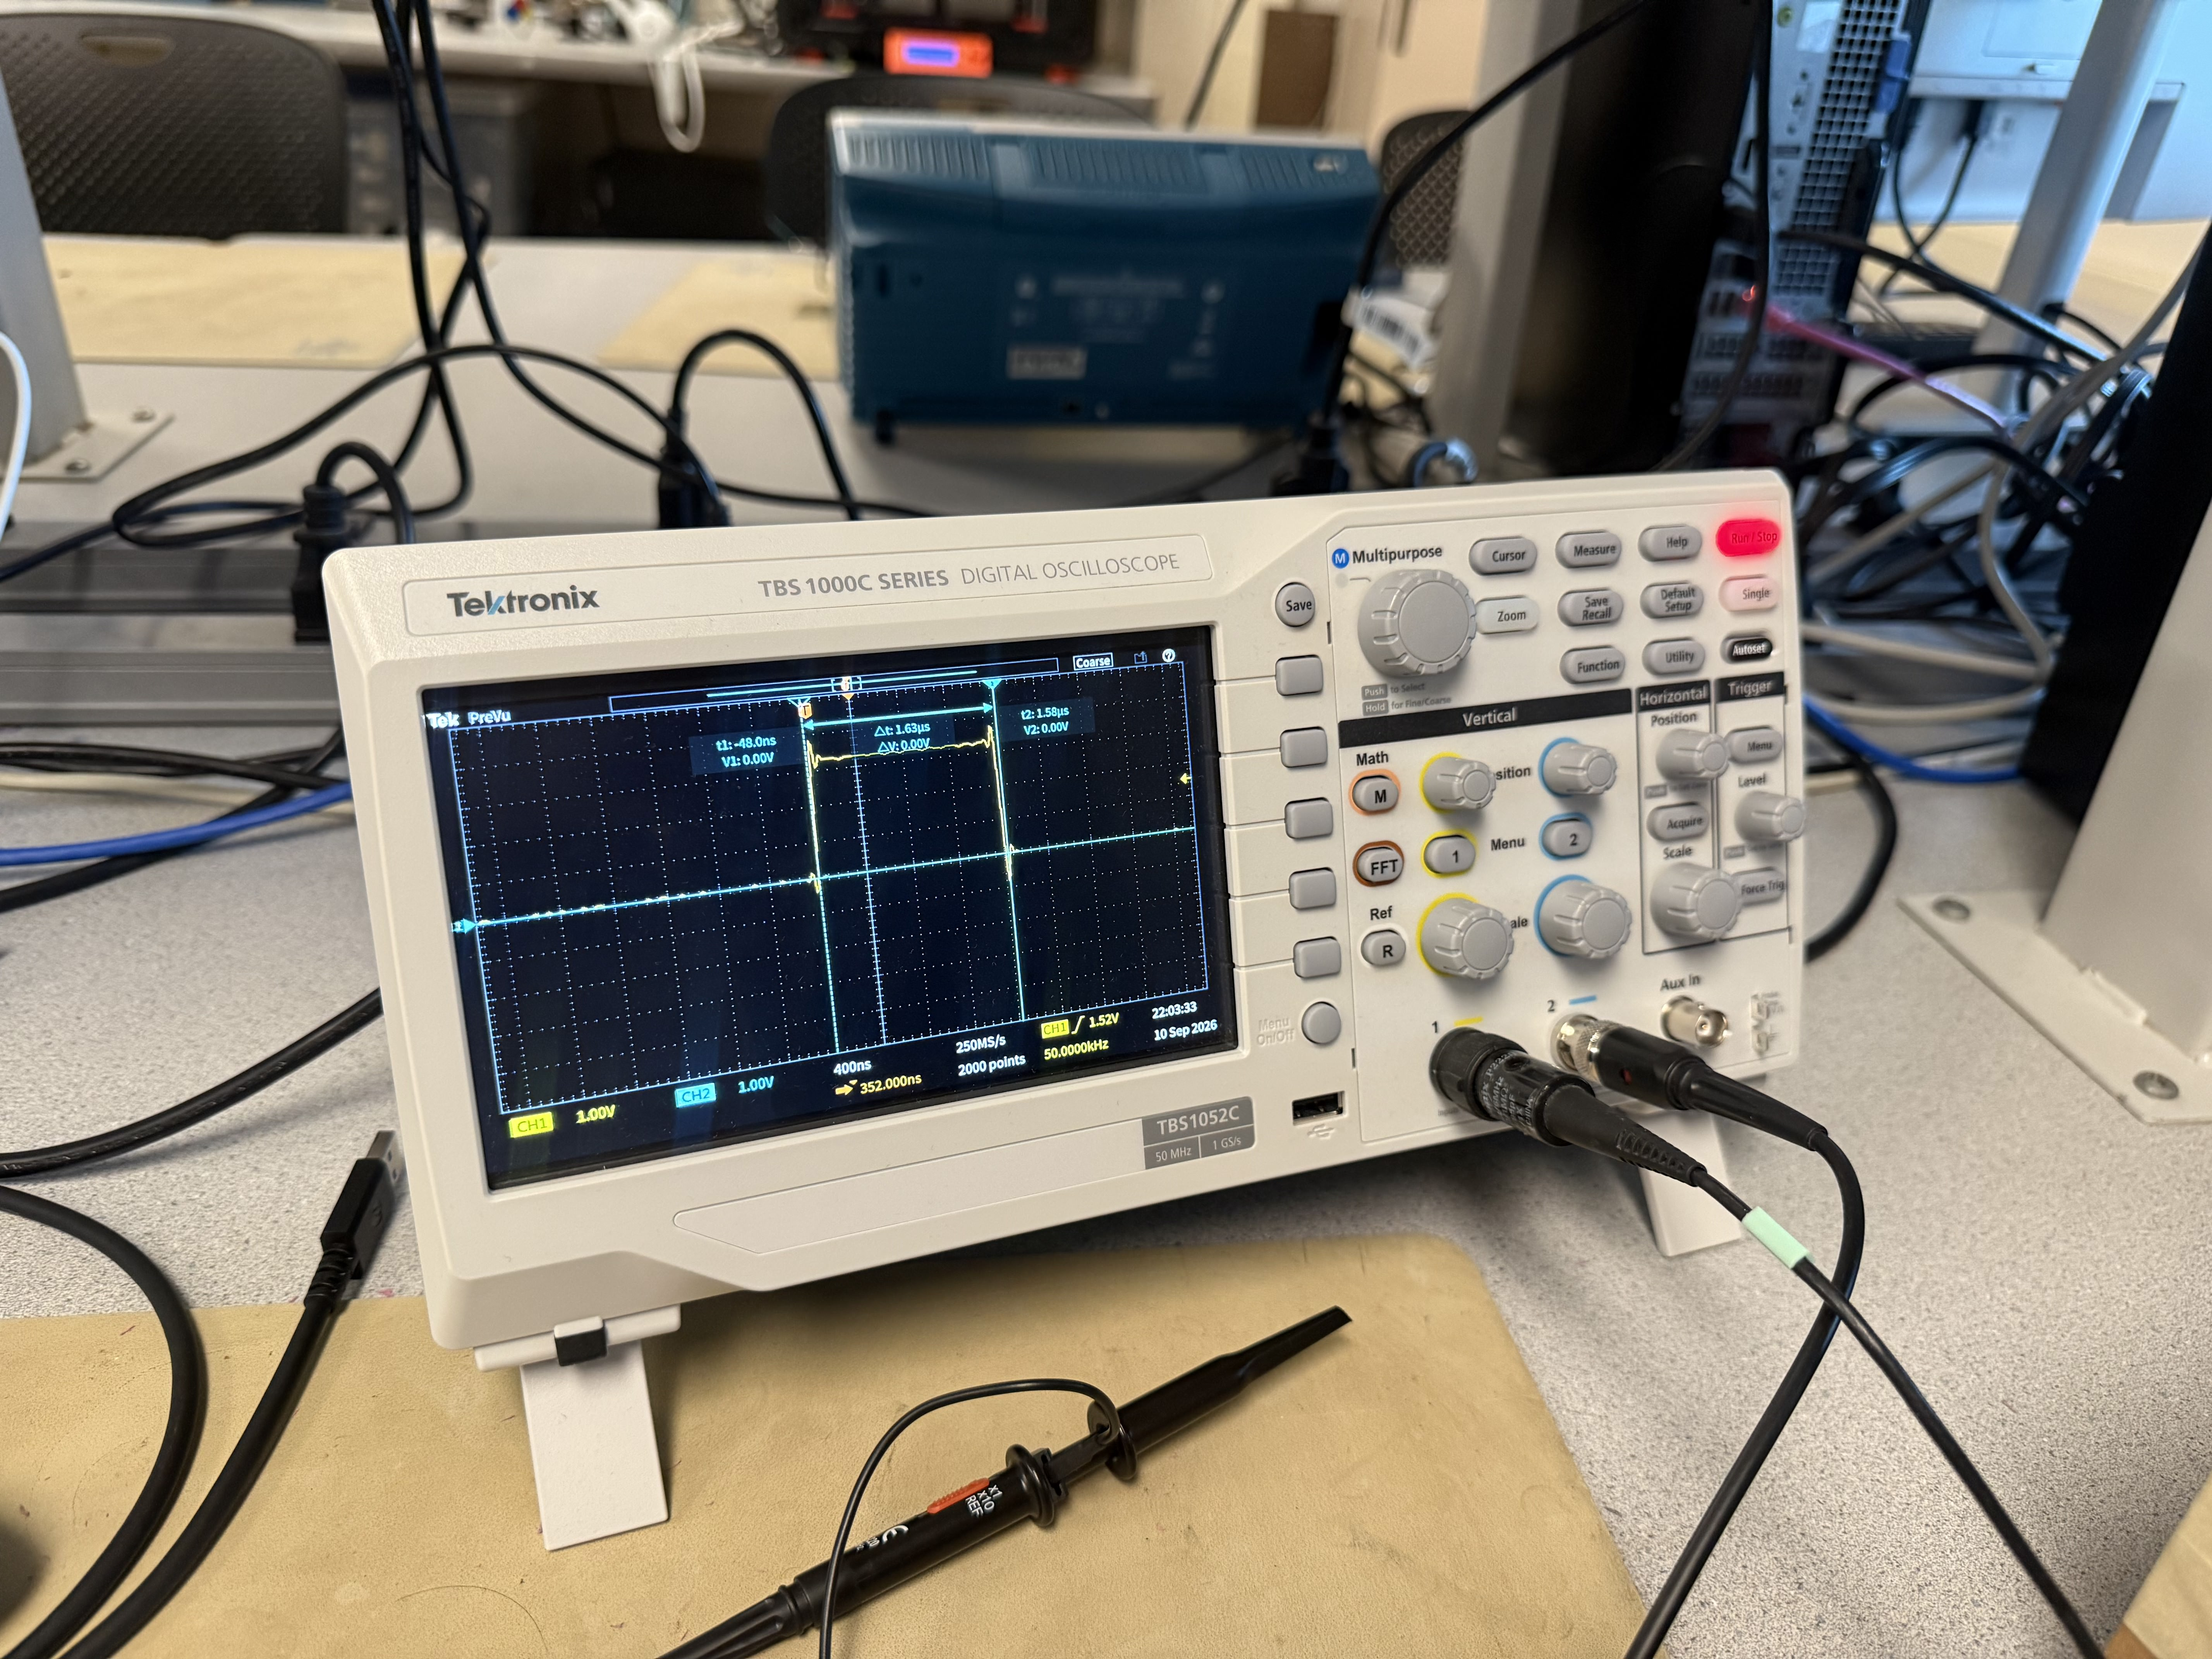
\includegraphics[width=\linewidth,height=0.65\textheight,keepaspectratio]{figures/isr_timing.jpg}
\caption{Timing-pulse oscilloscope capture with a 1.63 \ensuremath{\mu}s cursor separation and a 50.0000 kHz frequency readout. Horizontal scale: 400 ns/division. Photograph: IMG\_7909.}
\end{figure}

\textbf{Required envelope evidence:} [INSERT OSCILLOSCOPE CAPTURE of a complete generated sweep/chirp, labeling rise, sustain, fall, voltage scale, and time scale. The fixed-tone trace above does not show this envelope.]

\textbf{Required spectrogram:} [INSERT SPECTROGRAM of this device's audio, with time/frequency axes, recording method, and analysis settings.]

\subsection*{4.3 Limitations visible in the submitted snapshot}

Control actions are dispatched on confirmed press, despite the source comment and the requested press/release phrasing. Recording starts in the next held-key scan, introducing an extra scan interval after press confirmation, and stops after release confirmation. Short holds may not create new samples. The preserved write-length scheme does not explicitly clear the old slot length at the start of a new recording; a replacement that captures no samples can leave the previous sound intact.

The composition playback routine spends a separate iteration advancing between entries. During that roughly 1 ms interval, the DDS retains the previous frequency. Empty entries also consume an iteration, and an all-empty composition can briefly enable output at a stale frequency. The sequence-entry path accepts empty keys even though individual playback rejects them. A composition stores order only; pauses between the user's key presses are not recorded. Silence must be represented deliberately rather than inferred from entry timing.

Amplitude remains enabled between composition elements, so there is no independent attack/release envelope on each stored element. At the end of playback, clearing the playback flag lets the ADC thread regain frequency control before the fade necessarily finishes. These are identifiable limitations to compare with the scope and spectrogram, not measured claims that audible artifacts occurred.

\section*{5. Conclusions}

The saved implementation provides a compact architecture for a programmable birdsong instrument: a timer-driven DDS engine, low-rate frequency storage, accelerated replay, and a keypad composition interface. Separate source versions make the progression from basic DAC output to interactive synthesis reproducible. Previewing sounds during composition and using key 0 to return to the potentiometer reduce the need to reset or reprogram the board during use.

The principal engineering tradeoff is between simplicity and timing precision. Cooperative threads simplify control logic, but their requested intervals do not guarantee exact playback speed. Finite arrays avoid allocation complexity while limiting both sound duration and composition length. Boolean mode flags are workable when consistently reset, but an explicit mode enumeration and centralized transition functions would make future changes easier to verify.

Further improvements would include deadline-based frequency updates, suppression or throttling of diagnostic prints during timing measurements, explicit handling of empty/full buffers, and defined transitions between successive sound envelopes. The supplied photographs support baseline sinusoidal output and a short timing-pulse interval. A completed evaluation still requires the envelope capture, spectrogram, additional timing trials, and demonstration results; the available evidence does not establish full checkpoint compliance.

\section*{6. Lab-Specific Deliverables and Questions}

The current lab page does not give a separate numbered theory-question list. Its report-specific deliverables are the envelope scope capture, a generated-audio spectrogram, a commented program listing, and an AI prompt log with exchange and change counts. The results section includes the fixed-tone and timing photographs and identifies the envelope and spectrogram evidence still needed; Appendix A supplies the annotated listing; Appendix B supplies a partial AI provenance record and identifies the missing full export. \href{https://vanhunteradams.com/Pico/Birds/Birdsong.html}{Lab report instructions}.

For the timing question, compute interrupt occupancy from measured values as \texttt{100 \ensuremath{\times} ISR\_high\_time / measured\_period}. Report that the GPIO pulse omits overhead outside the instrumentation. For the acceleration question, use the measured duration ratio rather than multiplying the DDS phase increment. For the storage question, 100 Hz frequency storage is sufficient for the deliberately slow input trajectory and uses 1/500 the samples of 50 kHz waveform storage at equal sample width.

The example reports informed organization only: an explanation of design choices, diagrams linked to software, explicit testing methods, measured results, and a code appendix. Their hardware, experiments, measurements, and conclusions were not reused as this group's results. References: \href{https://vanhunteradams.com/Pico/CourseMaterials/Birdsong.pdf}{Birdsong}, \href{https://vanhunteradams.com/Pico/CourseMaterials/Birdsong2.pdf}{Birdsong2}, \href{https://vanhunteradams.com/Pico/CourseMaterials/cricket.pdf}{Cricket}, and \href{https://vanhunteradams.com/Pico/CourseMaterials/reaction.pdf}{Reaction}.

\section*{Submission Completion Checklist}

\begin{itemize}
\item Insert group names, dates, actual board identification, and demonstrated source version.
\item Add the as-built schematic, including latch, power, boot button, and audio connections.
\item Replace experimental placeholders with recorded results, not nominal values.
\item Add the waveform/envelope figure and spectrogram; confirm the probe connection and firmware used for the supplied timing trace.
\item Confirm checkpoint/demo outcomes and any Merlin identification result.
\item Export the complete AI conversation, reconcile suggested/accepted change counts, and attach it with Appendix B.
\item Reconcile the documented implementation limitations with the version actually demonstrated.
\end{itemize}

\clearpage
\section*{Appendix A: Annotated Source Snapshot}

Snapshot date: September 20, 2026. Original application files are unchanged. Comments marked REPORT NOTE were inserted only in the final-source listing below. Other source text is preserved. These notes explain behavior, not implemented fixes.

\begingroup\small
\setlength{\tabcolsep}{5pt}
\begin{longtable}{|>{\raggedright\arraybackslash}p{0.458\linewidth}|>{\raggedright\arraybackslash}p{0.458\linewidth}|}
\hline
\textbf{File} & \textbf{SHA-256 of original bytes} \\ \hline
\endhead
dactest.c & \seqsplit{cc4bc1069280c53bd303e90ed557e279c2094c1c9d0648b568e8e1117b79701e} \\ \hline
dactest\_other\_channel.c & \seqsplit{db55fd5c39fc7d93591a67f3af02b89bf2e392f994765fd3cda78612e6356906} \\ \hline
ADC\_with\_DDS.c & \seqsplit{3fc01390cb1ba028b35a32cbb4d661edfecb50ade77d1f5c9b18ae416890af19} \\ \hline
ADC\_DDS\_keypad\_mute.c & \seqsplit{669d9393b6a637c8b51e0ce2d6ae9fc89231432dbc44c26fcb4d360034178846} \\ \hline
ADC\_DDS\_keypad\_record.c & \seqsplit{6ea0fd24342e753c004fb8e74a9a648411303fd9e9ab400118e07ef4037f6c55} \\ \hline
ADC\_DDS\_keypad\_speedup.c & \seqsplit{bb1a61ee89eeca9226ba5d9b1199d1cd2c6f6714c88119244d862d7483b6ac75} \\ \hline
CMakeLists.txt & \seqsplit{abbacbd8c017fe768584f6b78d768bbd91732b4158c4b4a4c254a1e04fd141c6} \\ \hline
\end{longtable}
\endgroup

\section*{dactest.c}

Week 1 baseline: a fixed 800 Hz phase increment feeds channel A. The timer ISR performs the table lookup and SPI write.

\begin{lstlisting}[language=C]
/**
 * V. Hunter Adams
 * DDS of sine wave on MCP4822 DAC w/ ISR
 * 
 * Modified example code from Raspberry Pi
 * Copyright (c) 2020 Raspberry Pi (Trading) Ltd.
 *
 * SPDX-License-Identifier: BSD-3-Clause
 *
   GPIO 5 (pin 7) Chip select
   GPIO 6 (pin 9) SCK/spi0_sclk
   GPIO 7 (pin 10) MOSI/spi0_tx
   GPIO 2 (pin 4) GPIO output for timing ISR
   3.3v (pin 36) -> VCC on DAC 
   GND (pin 3)  -> GND on DAC 
 */

#include <stdio.h>
#include <math.h>
#include "pico/stdlib.h"
#include "hardware/timer.h"
#include "hardware/irq.h"
#include "hardware/spi.h"

// Low-level alarm infrastructure we'll be using
#define ALARM_NUM 0
#define ALARM_IRQ timer_hardware_alarm_get_irq_num(timer_hw, ALARM_NUM)

//DDS parameters
#define two32 4294967296.0 // 2^32 
#define Fs 50000
#define DELAY 20 // 1/Fs (in microseconds)
// the DDS units:
volatile unsigned int phase_accum_main;
volatile unsigned int phase_incr_main = (800.0*two32)/Fs ;

// SPI data
uint16_t DAC_data ; // output value

//DAC parameters
// A-channel, 1x, active
#define DAC_config_chan_A 0b0011000000000000
// B-channel, 1x, active
#define DAC_config_chan_B 0b1011000000000000

//SPI configurations
#define PIN_MISO 4
#define PIN_CS   5
#define PIN_SCK  6
#define PIN_MOSI 7
#define SPI_PORT spi0

//GPIO for timing the ISR
#define ISR_GPIO 2

// DDS sine table
#define sine_table_size 256
volatile int sin_table[sine_table_size] ;

// Alarm ISR
static void alarm_irq(void) {

    // Assert a GPIO when we enter the interrupt
    gpio_put(ISR_GPIO, 1) ;

    // Clear the alarm irq
    hw_clear_bits(&timer_hw->intr, 1u << ALARM_NUM);

    // Reset the alarm register
    timer_hw->alarm[ALARM_NUM] = timer_hw->timerawl + DELAY ;

	// DDS phase and sine table lookup
	phase_accum_main += phase_incr_main  ;
    DAC_data = (DAC_config_chan_A | ((sin_table[phase_accum_main>>24] + 2048) & 0xffff))  ;

    // Perform an SPI transaction
    spi_write16_blocking(SPI_PORT, &DAC_data, 1) ;

    // De-assert the GPIO when we leave the interrupt
    gpio_put(ISR_GPIO, 0) ;

}

int main() {
    // Initialize stdio
    stdio_init_all();
    printf("Hello, DAC!\n");

    // Initialize SPI channel (channel, baud rate set to 20MHz)
    spi_init(SPI_PORT, 20000000) ;
    // Format (channel, data bits per transfer, polarity, phase, order)
    spi_set_format(SPI_PORT, 16, 0, 0, 0);

    // Setup the ISR-timing GPIO
    gpio_init(ISR_GPIO) ;
    gpio_set_dir(ISR_GPIO, GPIO_OUT);
    gpio_put(ISR_GPIO, 0) ;

    // Map SPI signals to GPIO ports
    gpio_set_function(PIN_MISO, GPIO_FUNC_SPI);
    gpio_set_function(PIN_SCK, GPIO_FUNC_SPI);
    gpio_set_function(PIN_MOSI, GPIO_FUNC_SPI);
    gpio_set_function(PIN_CS, GPIO_FUNC_SPI) ;

    // === build the sine lookup table =======
   	// scaled to produce values between 0 and 4096
    int ii;
    for (ii = 0; ii < sine_table_size; ii++){
         sin_table[ii] = (int)(2047*sin((float)ii*6.283/(float)sine_table_size));
    }

    // Enable the interrupt for the alarm (we're using Alarm 0)
    hw_set_bits(&timer_hw->inte, 1u << ALARM_NUM) ;
    // Associate an interrupt handler with the ALARM_IRQ
    irq_set_exclusive_handler(ALARM_IRQ, alarm_irq) ;
    // Enable the alarm interrupt
    irq_set_enabled(ALARM_IRQ, true) ;
    // Write the lower 32 bits of the target time to the alarm register, arming it.
    timer_hw->alarm[ALARM_NUM] = timer_hw->timerawl + DELAY ;

    // Nothing happening here
    while(1){
    }
    return 0;
}
\end{lstlisting}


\section*{dactest\_other\_channel.c}

Week 1 channel experiment: the DAC control word selects B rather than A. The DDS frequency remains 800 Hz.

\begin{lstlisting}[language=C]
/**
 * V. Hunter Adams
 * DDS of sine wave on MCP4822 DAC w/ ISR
 * 
 * Modified example code from Raspberry Pi
 * Copyright (c) 2020 Raspberry Pi (Trading) Ltd.
 *
 * SPDX-License-Identifier: BSD-3-Clause
 *
   GPIO 5 (pin 7) Chip select
   GPIO 6 (pin 9) SCK/spi0_sclk
   GPIO 7 (pin 10) MOSI/spi0_tx
   GPIO 2 (pin 4) GPIO output for timing ISR
   3.3v (pin 36) -> VCC on DAC 
   GND (pin 3)  -> GND on DAC 
 */

#include <stdio.h>
#include <math.h>
#include "pico/stdlib.h"
#include "hardware/timer.h"
#include "hardware/irq.h"
#include "hardware/spi.h"

// Low-level alarm infrastructure we'll be using
#define ALARM_NUM 0
#define ALARM_IRQ timer_hardware_alarm_get_irq_num(timer_hw, ALARM_NUM)

//DDS parameters
#define two32 4294967296.0 // 2^32 
#define Fs 50000
#define DELAY 20 // 1/Fs (in microseconds)
// the DDS units:
volatile unsigned int phase_accum_main;
volatile unsigned int phase_incr_main = (800.0*two32)/Fs ;

// SPI data
uint16_t DAC_data ; // output value

//DAC parameters
// A-channel, 1x, active
#define DAC_config_chan_A 0b0011000000000000
// B-channel, 1x, active
#define DAC_config_chan_B 0b1011000000000000

//SPI configurations
#define PIN_MISO 4
#define PIN_CS   5
#define PIN_SCK  6
#define PIN_MOSI 7
#define SPI_PORT spi0

//GPIO for timing the ISR
#define ISR_GPIO 2

// DDS sine table
#define sine_table_size 256
volatile int sin_table[sine_table_size] ;

// Alarm ISR
static void alarm_irq(void) {

    // Assert a GPIO when we enter the interrupt
    gpio_put(ISR_GPIO, 1) ;

    // Clear the alarm irq
    hw_clear_bits(&timer_hw->intr, 1u << ALARM_NUM);

    // Reset the alarm register
    timer_hw->alarm[ALARM_NUM] = timer_hw->timerawl + DELAY ;

	// DDS phase and sine table lookup
	phase_accum_main += phase_incr_main  ;
    DAC_data = (DAC_config_chan_B | ((sin_table[phase_accum_main>>24] + 2048) & 0xffff))  ;

    // Perform an SPI transaction
    spi_write16_blocking(SPI_PORT, &DAC_data, 1) ;

    // De-assert the GPIO when we leave the interrupt
    gpio_put(ISR_GPIO, 0) ;

}

int main() {
    // Initialize stdio
    stdio_init_all();
    printf("Hello, DAC!\n");

    // Initialize SPI channel (channel, baud rate set to 20MHz)
    spi_init(SPI_PORT, 20000000) ;
    // Format (channel, data bits per transfer, polarity, phase, order)
    spi_set_format(SPI_PORT, 16, 0, 0, 0);

    // Setup the ISR-timing GPIO
    gpio_init(ISR_GPIO) ;
    gpio_set_dir(ISR_GPIO, GPIO_OUT);
    gpio_put(ISR_GPIO, 0) ;

    // Map SPI signals to GPIO ports
    gpio_set_function(PIN_MISO, GPIO_FUNC_SPI);
    gpio_set_function(PIN_SCK, GPIO_FUNC_SPI);
    gpio_set_function(PIN_MOSI, GPIO_FUNC_SPI);
    gpio_set_function(PIN_CS, GPIO_FUNC_SPI) ;

    // === build the sine lookup table =======
   	// scaled to produce values between 0 and 4096
    int ii;
    for (ii = 0; ii < sine_table_size; ii++){
         sin_table[ii] = (int)(2047*sin((float)ii*6.283/(float)sine_table_size));
    }

    // Enable the interrupt for the alarm (we're using Alarm 0)
    hw_set_bits(&timer_hw->inte, 1u << ALARM_NUM) ;
    // Associate an interrupt handler with the ALARM_IRQ
    irq_set_exclusive_handler(ALARM_IRQ, alarm_irq) ;
    // Enable the alarm interrupt
    irq_set_enabled(ALARM_IRQ, true) ;
    // Write the lower 32 bits of the target time to the alarm register, arming it.
    timer_hw->alarm[ALARM_NUM] = timer_hw->timerawl + DELAY ;

    // Nothing happening here
    while(1){
    }
    return 0;
}
\end{lstlisting}


\section*{ADC\_with\_DDS.c}

Week 1 integration: the ADC thread converts a potentiometer code to Hz, then to a phase increment. The timer ISR independently emits audio samples.

\begin{lstlisting}[language=C]

/*
Simple ADC/Protothreads demo

Schedules a single thread, reads/prints ADC value

 */

#include "hardware/gpio.h"
#include "hardware/timer.h"
#include "hardware/adc.h"
#include "pico/stdlib.h"
#include <stdio.h>
#include <string.h>
#include "stdlib.h"
#include "hardware/spi.h"
#include <math.h>
#include "hardware/irq.h"

// ==========================================
// === protothreads globals
// ==========================================
// protothreads header
#include "pt_cornell_rp2040_v1_4.h"

#define LED_PIN 25
#define ADC_PIN 26
#define ADC_MUX 0

// Low-level alarm infrastructure we'll be using
#define ALARM_NUM 0
#define ALARM_IRQ timer_hardware_alarm_get_irq_num(timer_hw, ALARM_NUM)

//DDS parameters
#define two32 4294967296.0 // 2^32 
#define Fs 50000
#define DELAY 20 // 1/Fs (in microseconds)
// the DDS units:
volatile unsigned int phase_accum_main;
volatile unsigned int phase_incr_main;

// SPI data
uint16_t DAC_data ; // output value

//DAC parameters
// A-channel, 1x, active
#define DAC_config_chan_A 0b0011000000000000
// B-channel, 1x, active
#define DAC_config_chan_B 0b1011000000000000

//SPI configurations
#define PIN_MISO 4
#define PIN_CS   5
#define PIN_SCK  6
#define PIN_MOSI 7
#define SPI_PORT spi0

//GPIO for timing the ISR
#define ISR_GPIO 2

// DDS sine table
#define sine_table_size 256
volatile int sin_table[sine_table_size] ;

volatile static unsigned int adc_val ;

static int map(int x, int in_min, int in_max, int out_min, int out_max) {
    return (x - in_min) * (out_max - out_min) / (in_max - in_min) + out_min;
}

// ==================================================
// === toggle25 thread 
// ==================================================
//  
static PT_THREAD (protothread_toggle25(struct pt *pt))
{
    PT_BEGIN(pt);

      while(1) {
        // toggle gpio 25
        gpio_put(LED_PIN, !gpio_get(LED_PIN));

        // Read the ADC
        adc_val = adc_read() ;

        phase_incr_main = (map(adc_val, 0, 4095, 0, 10000)*two32)/Fs;

        // Print the value
        printf("ADC value: %d\n", adc_val) ;

        // Yield
        PT_YIELD_usec(10000) ; //yeild every 10 ms
      } // END WHILE(1)
      // every thread ends with PT_END(pt);
      PT_END(pt);
} // end blink thread

// Alarm ISR
static void alarm_irq(void) {

    // Assert a GPIO when we enter the interrupt
    gpio_put(ISR_GPIO, 1) ;

    // Clear the alarm irq
    hw_clear_bits(&timer_hw->intr, 1u << ALARM_NUM);

    // Reset the alarm register
    timer_hw->alarm[ALARM_NUM] = timer_hw->timerawl + DELAY ; 

    // DDS phase and sine table lookup
    phase_accum_main += phase_incr_main  ;
    DAC_data = (DAC_config_chan_A | ((sin_table[phase_accum_main>>24] + 2048) & 0xffff))  ;

    // Perform an SPI transaction
    spi_write16_blocking(SPI_PORT, &DAC_data, 1) ;

    // De-assert the GPIO when we leave the interrupt
    gpio_put(ISR_GPIO, 0) ;

}

// ========================================
// === core 0 main
// ========================================
int main(){
  //===  start the serial i/o ==================
  stdio_init_all() ;
  // announce the threader version on system reset
  // if there is a seral terminal attached
  printf("\n\rProtothreads RP2040 v1.4\n\r");

  // Setup the ADC
  adc_init() ;
  adc_gpio_init(ADC_PIN) ;
  adc_select_input(ADC_MUX) ;

  // Initialize stdio
    stdio_init_all();
    printf("Hello, DAC!\n");

    // Initialize SPI channel (channel, baud rate set to 20MHz)
    spi_init(SPI_PORT, 20000000) ;
    // Format (channel, data bits per transfer, polarity, phase, order)
    spi_set_format(SPI_PORT, 16, 0, 0, 0);

    // Setup the ISR-timing GPIO
    gpio_init(ISR_GPIO) ;
    gpio_set_dir(ISR_GPIO, GPIO_OUT);
    gpio_put(ISR_GPIO, 0) ;

    // Map SPI signals to GPIO ports
    gpio_set_function(PIN_MISO, GPIO_FUNC_SPI);
    gpio_set_function(PIN_SCK, GPIO_FUNC_SPI);
    gpio_set_function(PIN_MOSI, GPIO_FUNC_SPI);
    gpio_set_function(PIN_CS, GPIO_FUNC_SPI) ;

    // === build the sine lookup table =======
   	// scaled to produce values between 0 and 4096
    int ii;
    for (ii = 0; ii < sine_table_size; ii++){
         sin_table[ii] = (int)(2047*sin((float)ii*6.283/(float)sine_table_size));
    }

        // Enable the interrupt for the alarm (we're using Alarm 0)
    hw_set_bits(&timer_hw->inte, 1u << ALARM_NUM) ;
    // Associate an interrupt handler with the ALARM_IRQ
    irq_set_exclusive_handler(ALARM_IRQ, alarm_irq) ;
    // Enable the alarm interrupt
    irq_set_enabled(ALARM_IRQ, true) ;
    // Write the lower 32 bits of the target time to the alarm register, arming it.
    timer_hw->alarm[ALARM_NUM] = timer_hw->timerawl + DELAY ;

  // set up LED gpio 25
  gpio_init(LED_PIN) ;  
  gpio_set_dir(LED_PIN, GPIO_OUT) ;
  gpio_put(LED_PIN, true);

  // === config threads ========================
  pt_add_thread(protothread_toggle25);
  
  // === initalize the scheduler ===============
  pt_schedule_start ;

    // Nothing happening here
    while(1){
    }
    return 0;
} // end main
\end{lstlisting}


\section*{ADC\_DDS\_keypad\_mute.c}

Week 2 mute stage: keypad scanning and a four-state debounce machine set tone\_enabled; the amplitude thread ramps output rather than rebuilding the sine table.

\begin{lstlisting}[language=C]

/*
Simple ADC/Protothreads demo

Schedules a single thread, reads/prints ADC value

 */

#include "hardware/gpio.h"
#include "hardware/timer.h"
#include "hardware/adc.h"
#include "pico/stdlib.h"
#include "pico/multicore.h"
#include <stdio.h>
#include <string.h>
#include "stdlib.h"
#include "hardware/spi.h"
#include <math.h>
#include "hardware/irq.h"
#include "hardware/pio.h"
#include "hardware/dma.h"
#include "hardware/sync.h"
#include "hardware/spi.h"
#include "hardware/clocks.h"

// ==========================================
// === protothreads globals
// ==========================================
// protothreads header
#include "pt_cornell_rp2040_v1_4.h"

#define LED_PIN 25
#define ADC_PIN 26
#define ADC_MUX 0

// Low-level alarm infrastructure we'll be using
#define ALARM_NUM 0
#define ALARM_IRQ timer_hardware_alarm_get_irq_num(timer_hw, ALARM_NUM)

//DDS parameters
#define two32 4294967296.0 // 2^32 
#define Fs 50000
#define DELAY 20 // 1/Fs (in microseconds)

//keypad constants
#define BASE_KEYPAD_PIN 9
#define KEYROWS         4
#define NUMKEYS         12
// the DDS units:
volatile unsigned int phase_accum_main;
volatile unsigned int phase_incr_main;

// SPI data
uint16_t DAC_data ; // output value

//DAC parameters
// A-channel, 1x, active
#define DAC_config_chan_A 0b0011000000000000
// B-channel, 1x, active
#define DAC_config_chan_B 0b1011000000000000

//SPI configurations
#define PIN_MISO 4
#define PIN_CS   5
#define PIN_SCK  6
#define PIN_MOSI 7
#define SPI_PORT spi0

//GPIO for timing the ISR
#define ISR_GPIO 2

// DDS sine table
#define sine_table_size 256
volatile int sin_table[sine_table_size] ;

volatile static unsigned int adc_val ;

static int map(int x, int in_min, int in_max, int out_min, int out_max) {
    return (x - in_min) * (out_max - out_min) / (in_max - in_min) + out_min;
}

//keycodes
unsigned int keycodes[NUMKEYS] = {      0x57, 0x6E, 0x5E, 0x3E, 0x6D,
                                        0x5D, 0x3D, 0x6B, 0x5B, 0x3B,
                                        0x67, 0x37} ;
unsigned int scancodes[KEYROWS] = {   0xE, 0xD, 0xB, 0x7} ;
unsigned int button = 0x70 ;
char keytext[40];
int prev_key = 0;

//muting variables
#define AMPLITUDE_STEP 103 // 20 updates at 1 ms each for a full fade
volatile bool tone_enabled = true;
volatile int amplitude = 2047; // 0 = silent, 2047 = full amplitude

//debouncing states
#define NOT_PRESSED 0
#define MAYBE_PRESSED 1
#define PRESSED 2
#define MAYBE_NOT_PRESSED 3


// ==================================================
// === toggle25 thread 
// ==================================================
//  
static PT_THREAD (protothread_toggle25(struct pt *pt))
{
    PT_BEGIN(pt);

      while(1) {
        // toggle gpio 25
        gpio_put(LED_PIN, !gpio_get(LED_PIN));

        // Read the ADC
        adc_val = adc_read() ;

        phase_incr_main = (map(adc_val, 0, 4095, 0, 10000)*two32)/Fs;

        // Print the value
        printf("ADC value: %d\n", adc_val) ;

        // Yield
        PT_YIELD_usec(10000) ; //yeild every 10 ms
      } // END WHILE(1)
      // every thread ends with PT_END(pt);
      PT_END(pt);
} // end blink thread

// This thread runs on core 0
static PT_THREAD (protothread_core_0(struct pt *pt))
{
    // Indicate thread beginning
    PT_BEGIN(pt) ;

    // Some variables
    static int i ;
    static uint32_t keypad ;
    static int possible;
    static int state;

    while(1) {

        // Scan the keypad!
        for (i=0; i<KEYROWS; i++) {
            // Set a row high
            gpio_put_masked((0xF << BASE_KEYPAD_PIN),
                            (scancodes[i] << BASE_KEYPAD_PIN)) ;
            // Small delay required
            sleep_us(1) ;
            // Read the keycode
            keypad = ((gpio_get_all() >> BASE_KEYPAD_PIN) & 0x7F) ;
            // Break if button(s) are pressed
            if ((~keypad) & button) break ;
        }
        // If we found a button . . .
        if ((~keypad) & button) {
            // Look for a valid keycode.
            for (i=0; i<NUMKEYS; i++) {
                if (keypad == keycodes[i]) break ;
            }
            // If we don't find one, report invalid keycode
            if (i==NUMKEYS) (i = -1) ;
        }
        // Otherwise, indicate invalid/non-pressed buttons
        else (i=-1) ;

        switch (state) {

          case NOT_PRESSED:
            if (i != -1) {
              possible = i;
              state = MAYBE_PRESSED;
            }
            break;

          case MAYBE_PRESSED:
            if (i == possible){
              state = PRESSED;
              // Toggle once on confirmed release of the remembered key.
              if (possible == 0) {
                tone_enabled = !tone_enabled;
              // Print key to terminal
              printf("\n%d", i) ;
              }
            }
            else {
              state = NOT_PRESSED;
            }
            break;
          
          case PRESSED:
            if (i == possible){
              state = PRESSED;
            }
            else {
              state = MAYBE_NOT_PRESSED;
            }
            break;

          case MAYBE_NOT_PRESSED:
            if (i == possible){
              state = PRESSED;
            }
            else {
              state = NOT_PRESSED;
              }
            break;

          default:
            state = NOT_PRESSED;
            break;

        }

        PT_YIELD_usec(30000) ;
    }
    // Indicate thread end
    PT_END(pt) ;
}

// This thread runs on core 0
static PT_THREAD (protothread_amplitude(struct pt *pt))
{
    // Indicate thread beginning
    PT_BEGIN(pt) ;

    while (1){

      if (tone_enabled && amplitude < 2047){
        int next_amplitude = amplitude + AMPLITUDE_STEP;
        amplitude = (next_amplitude > 2047) ? 2047 : next_amplitude;
      }

      else if (!tone_enabled && amplitude > 0){
        int next_amplitude = amplitude - AMPLITUDE_STEP;
        amplitude = (next_amplitude < 0) ? 0 : next_amplitude;
      }

      PT_YIELD_usec(1000) ;
    }

    PT_END(pt) ;

}

// Alarm ISR
static void alarm_irq(void) {

    // Assert a GPIO when we enter the interrupt
    gpio_put(ISR_GPIO, 1) ;

    // Clear the alarm irq
    hw_clear_bits(&timer_hw->intr, 1u << ALARM_NUM);

    // Reset the alarm register
    timer_hw->alarm[ALARM_NUM] = timer_hw->timerawl + DELAY ; 

    // DDS phase and sine table lookup
    phase_accum_main += phase_incr_main  ;
    DAC_data = (DAC_config_chan_A | (((sin_table[phase_accum_main>>24] * amplitude)/2047 + 2048) & 0xffff))  ;

    // Perform an SPI transaction
    spi_write16_blocking(SPI_PORT, &DAC_data, 1) ;

    // De-assert the GPIO when we leave the interrupt
    gpio_put(ISR_GPIO, 0) ;

}

// ========================================
// === core 0 main
// ========================================
int main(){
  //===  start the serial i/o ==================
  stdio_init_all() ;
  // announce the threader version on system reset
  // if there is a seral terminal attached
  printf("\n\rProtothreads RP2040 v1.4\n\r");

  // Setup the ADC
  adc_init() ;
  adc_gpio_init(ADC_PIN) ;
  adc_select_input(ADC_MUX) ;

  // Initialize stdio
  stdio_init_all();
  printf("Hello, DAC!\n");

  // Initialize SPI channel (channel, baud rate set to 20MHz)
  spi_init(SPI_PORT, 20000000) ;
  // Format (channel, data bits per transfer, polarity, phase, order)
  spi_set_format(SPI_PORT, 16, 0, 0, 0);

  // Setup the ISR-timing GPIO
  gpio_init(ISR_GPIO) ;
  gpio_set_dir(ISR_GPIO, GPIO_OUT);
  gpio_put(ISR_GPIO, 0) ;

  // Map SPI signals to GPIO ports
  gpio_set_function(PIN_MISO, GPIO_FUNC_SPI);
  gpio_set_function(PIN_SCK, GPIO_FUNC_SPI);
  gpio_set_function(PIN_MOSI, GPIO_FUNC_SPI);
  gpio_set_function(PIN_CS, GPIO_FUNC_SPI) ;

  // === build the sine lookup table =======
  // scaled to produce values between 0 and 4096
  int ii;
  for (ii = 0; ii < sine_table_size; ii++){
        sin_table[ii] = (int)(2047*sin((float)ii*6.283/(float)sine_table_size));
  }

      // Enable the interrupt for the alarm (we're using Alarm 0)
  hw_set_bits(&timer_hw->inte, 1u << ALARM_NUM) ;
  // Associate an interrupt handler with the ALARM_IRQ
  irq_set_exclusive_handler(ALARM_IRQ, alarm_irq) ;
  // Enable the alarm interrupt
  irq_set_enabled(ALARM_IRQ, true) ;
  // Write the lower 32 bits of the target time to the alarm register, arming it.
  timer_hw->alarm[ALARM_NUM] = timer_hw->timerawl + DELAY ;

  // set up LED gpio 25
  gpio_init(LED_PIN) ;  
  gpio_set_dir(LED_PIN, GPIO_OUT) ;
  gpio_put(LED_PIN, true);

    ////////////////// KEYPAD INITS ///////////////////////
  // Initialize the keypad GPIO's
  gpio_init_mask((0x7F << BASE_KEYPAD_PIN)) ;
  gpio_set_dir((BASE_KEYPAD_PIN+4), GPIO_IN);
  gpio_set_dir((BASE_KEYPAD_PIN+5), GPIO_IN);
  gpio_set_dir((BASE_KEYPAD_PIN+6), GPIO_IN);
  // Set row-pins to output
  gpio_set_dir_out_masked((0xF << BASE_KEYPAD_PIN)) ;
  // Set all output pins to low
  gpio_put_masked((0xF << BASE_KEYPAD_PIN), (0xF << BASE_KEYPAD_PIN)) ;
  // Turn on pulldown resistors for column pins (on by default)
  gpio_pull_up((BASE_KEYPAD_PIN+4)) ;
  gpio_pull_up((BASE_KEYPAD_PIN+5)) ;
  gpio_pull_up((BASE_KEYPAD_PIN+6)) ;

  // === config threads ========================
  pt_add_thread(protothread_toggle25);
  pt_add_thread(protothread_core_0);
  pt_add_thread(protothread_amplitude);
  
  // === initalize the scheduler ===============
  pt_schedule_start ;

  // Nothing happening here
  while(1){
  }
  return 0;
} // end main
\end{lstlisting}


\section*{ADC\_DDS\_keypad\_record.c}

Week 2 recording stage: nine buffers store frequencies in Hz. The recording and playback threads both request 10 ms intervals. Historical snapshot, not the current build target.

\begin{lstlisting}[language=C]

/*
Simple ADC/Protothreads demo

Schedules a single thread, reads/prints ADC value

 */

#include "hardware/gpio.h"
#include "hardware/timer.h"
#include "hardware/adc.h"
#include "pico/stdlib.h"
#include "pico/multicore.h"
#include <stdio.h>
#include <string.h>
#include "stdlib.h"
#include "hardware/spi.h"
#include <math.h>
#include "hardware/irq.h"
#include "hardware/pio.h"
#include "hardware/dma.h"
#include "hardware/sync.h"
#include "hardware/spi.h"
#include "hardware/clocks.h"

// ==========================================
// === protothreads globals
// ==========================================
// protothreads header
#include "pt_cornell_rp2040_v1_4.h"

#define LED_PIN 25
#define ADC_PIN 26
#define ADC_MUX 0

// Low-level alarm infrastructure we'll be using
#define ALARM_NUM 0
#define ALARM_IRQ timer_hardware_alarm_get_irq_num(timer_hw, ALARM_NUM)

//DDS parameters
#define two32 4294967296.0 // 2^32 
#define Fs 50000
#define DELAY 20 // 1/Fs (in microseconds)

//keypad constants
#define BASE_KEYPAD_PIN 9
#define KEYROWS         4
#define NUMKEYS         12
// the DDS units:
volatile unsigned int phase_accum_main;
volatile unsigned int phase_incr_main;

// SPI data
uint16_t DAC_data ; // output value

//DAC parameters
// A-channel, 1x, active
#define DAC_config_chan_A 0b0011000000000000
// B-channel, 1x, active
#define DAC_config_chan_B 0b1011000000000000

//SPI configurations
#define PIN_MISO 4
#define PIN_CS   5
#define PIN_SCK  6
#define PIN_MOSI 7
#define SPI_PORT spi0

//GPIO for timing the ISR
#define ISR_GPIO 2

// DDS sine table
#define sine_table_size 256
volatile int sin_table[sine_table_size] ;

volatile static unsigned int adc_val ;

static int map(int x, int in_min, int in_max, int out_min, int out_max) {
    return (x - in_min) * (out_max - out_min) / (in_max - in_min) + out_min;
}

//keycodes
unsigned int keycodes[NUMKEYS] = {      0x57, 0x6E, 0x5E, 0x3E, 0x6D,
                                        0x5D, 0x3D, 0x6B, 0x5B, 0x3B,
                                        0x67, 0x37} ;
unsigned int scancodes[KEYROWS] = {   0xE, 0xD, 0xB, 0x7} ;
unsigned int button = 0x70 ;
char keytext[40];
int prev_key = 0;

//muting variables
#define AMPLITUDE_STEP 103 // 20 updates at 1 ms each for a full fade
volatile bool tone_enabled = false;
volatile int amplitude = 0; // 0 = silent, 2047 = full amplitude

//record variables

#define RECORD_HZ 100
#define MAX_SAMPLES (10 * RECORD_HZ)

volatile bool record_mode = false;
volatile bool record = false;
volatile bool play = false;
volatile int record_button = -1;
volatile int play_button = -1;
volatile int play_index = 0;
volatile uint16_t sounds[9][MAX_SAMPLES];
static unsigned int sound_length[9] = {0};

//debouncing states
#define NOT_PRESSED 0
#define MAYBE_PRESSED 1
#define PRESSED 2
#define MAYBE_NOT_PRESSED 3


// ==================================================
// === toggle25 thread 
// ==================================================
//  
static PT_THREAD (protothread_toggle25(struct pt *pt))
{
    PT_BEGIN(pt);

      while(1) {
        // toggle gpio 25
        gpio_put(LED_PIN, !gpio_get(LED_PIN));

        // Read the ADC
        adc_val = adc_read() ;

        if (!play){
          phase_incr_main = (map(adc_val, 0, 4095, 0, 10000)*two32)/Fs;
        }
        

        // Print the value
        //printf("ADC value: %d\n", adc_val) ;

        // Yield
        PT_YIELD_usec(10000) ; //yeild every 10 ms
      } // END WHILE(1)
      // every thread ends with PT_END(pt);
      PT_END(pt);
} // end blink thread

// This thread runs on core 0
static PT_THREAD (protothread_core_0(struct pt *pt))
{
    // Indicate thread beginning
    PT_BEGIN(pt) ;

    // Some variables
    static int i ;
    static uint32_t keypad ;
    static int possible;
    static int state;

    while(1) {

        // Scan the keypad!
        for (i=0; i<KEYROWS; i++) {
            // Set a row high
            gpio_put_masked((0xF << BASE_KEYPAD_PIN),
                            (scancodes[i] << BASE_KEYPAD_PIN)) ;
            // Small delay required
            sleep_us(1) ;
            // Read the keycode
            keypad = ((gpio_get_all() >> BASE_KEYPAD_PIN) & 0x7F) ;
            // Break if button(s) are pressed
            if ((~keypad) & button) break ;
        }
        // If we found a button . . .
        if ((~keypad) & button) {
            // Look for a valid keycode.
            for (i=0; i<NUMKEYS; i++) {
                if (keypad == keycodes[i]) break ;
            }
            // If we don't find one, report invalid keycode
            if (i==NUMKEYS) (i = -1) ;
        }
        // Otherwise, indicate invalid/non-pressed buttons
        else (i=-1) ;

        switch (state) {

          case NOT_PRESSED:
            if (i != -1) {
              possible = i;
              state = MAYBE_PRESSED;
            }
            break;

          case MAYBE_PRESSED:
            if (i == possible){
              state = PRESSED;
              // Toggle once on confirmed release of the remembered key.
              if (possible == 0) {
                tone_enabled = !tone_enabled;
              ;
              }

              if (possible == 10){
                record_mode = true;
                play = false;
              }

              if (!record_mode && (possible <=9 && possible >= 1)){
                play = true;
                play_button = possible;
                play_index = 0;
                tone_enabled = true;
              }
              // Print key to terminal
              printf("\n%d", i); 
            }
            else {
              state = NOT_PRESSED;
            }
            break;
          
          case PRESSED:
            if (i == possible){
              state = PRESSED;
              if (record_mode && (possible <=9 && possible >= 1)){
                record_button = possible;
                record = true;
              }
            }
            else {
              state = MAYBE_NOT_PRESSED;
            }
            break;

          case MAYBE_NOT_PRESSED:
            if (i == possible){
              state = PRESSED;
            }
            else {
              state = NOT_PRESSED;
              if (record_mode && possible == record_button){
                record_mode = false;
                record = false;
                record_button = -1;
              }
              }
            break;

          default:
            state = NOT_PRESSED;
            break;

        }

        PT_YIELD_usec(30000) ;
    }
    // Indicate thread end
    PT_END(pt) ;
}

// This thread ramps up/down amplitude of output wave
static PT_THREAD (protothread_amplitude(struct pt *pt))
{
    // Indicate thread beginning
    PT_BEGIN(pt) ;

    while (1){

      if (tone_enabled && amplitude < 2047){
        int next_amplitude = amplitude + AMPLITUDE_STEP;
        amplitude = (next_amplitude > 2047) ? 2047 : next_amplitude;
      }

      else if (!tone_enabled && amplitude > 0){
        int next_amplitude = amplitude - AMPLITUDE_STEP;
        amplitude = (next_amplitude < 0) ? 0 : next_amplitude;
      }

      PT_YIELD_usec(1000) ;
    }

    PT_END(pt) ;

}

// This thread handkes playback
static PT_THREAD (protothread_playback(struct pt *pt))
{
    // Indicate thread beginning
    PT_BEGIN(pt) ;

    while (1){

      if (play){
        if (play_index < sound_length[play_button - 1]) {
          uint16_t frequency = sounds[play_button - 1][play_index++];

          phase_incr_main = (unsigned int)((frequency * two32) / Fs);
        }
        else {
          play_index = 0;
          play = false;
          tone_enabled = false;
        }
      }
      else{
        play_index = 0;
      }

      PT_YIELD_usec(10000) ;
    }

    PT_END(pt) ;

}

static PT_THREAD (protothread_recording(struct pt *pt))
{
    // Indicate thread beginning
    PT_BEGIN(pt) ;

    static int length = 0;

    while (1){

      if (record){

        if(record_button != -1 && length < MAX_SAMPLES){
          sounds[record_button - 1][length] = (uint16_t)map(adc_val, 0, 4095, 0, 10000);;
          length++;
          sound_length[record_button - 1] = length;
        }
      }
      else{
        length = 0;
      }


      PT_YIELD_usec(10000) ;
    }

    PT_END(pt) ;

}

// Alarm ISR
static void alarm_irq(void) {

    // Assert a GPIO when we enter the interrupt
    gpio_put(ISR_GPIO, 1) ;

    // Clear the alarm irq
    hw_clear_bits(&timer_hw->intr, 1u << ALARM_NUM);

    // Reset the alarm register
    timer_hw->alarm[ALARM_NUM] = timer_hw->timerawl + DELAY ; 

    // DDS phase and sine table lookup
    phase_accum_main += phase_incr_main  ;

    DAC_data = (DAC_config_chan_A | (((sin_table[phase_accum_main>>24] * amplitude)/2047 + 2048) & 0xffff))  ;

    // Perform an SPI transaction
    spi_write16_blocking(SPI_PORT, &DAC_data, 1) ;

    // De-assert the GPIO when we leave the interrupt
    gpio_put(ISR_GPIO, 0) ;

}

// ========================================
// === core 0 main
// ========================================
int main(){
  //===  start the serial i/o ==================
  stdio_init_all() ;
  // announce the threader version on system reset
  // if there is a seral terminal attached
  printf("\n\rProtothreads RP2040 v1.4\n\r");

  // Setup the ADC
  adc_init() ;
  adc_gpio_init(ADC_PIN) ;
  adc_select_input(ADC_MUX) ;

  // Initialize stdio
  stdio_init_all();
  printf("Hello, DAC!\n");

  // Initialize SPI channel (channel, baud rate set to 20MHz)
  spi_init(SPI_PORT, 20000000) ;
  // Format (channel, data bits per transfer, polarity, phase, order)
  spi_set_format(SPI_PORT, 16, 0, 0, 0);

  // Setup the ISR-timing GPIO
  gpio_init(ISR_GPIO) ;
  gpio_set_dir(ISR_GPIO, GPIO_OUT);
  gpio_put(ISR_GPIO, 0) ;

  // Map SPI signals to GPIO ports
  gpio_set_function(PIN_MISO, GPIO_FUNC_SPI);
  gpio_set_function(PIN_SCK, GPIO_FUNC_SPI);
  gpio_set_function(PIN_MOSI, GPIO_FUNC_SPI);
  gpio_set_function(PIN_CS, GPIO_FUNC_SPI) ;

  // === build the sine lookup table =======
  // scaled to produce values between 0 and 4096
  int ii;
  for (ii = 0; ii < sine_table_size; ii++){
        sin_table[ii] = (int)(2047*sin((float)ii*6.283/(float)sine_table_size));
  }

      // Enable the interrupt for the alarm (we're using Alarm 0)
  hw_set_bits(&timer_hw->inte, 1u << ALARM_NUM) ;
  // Associate an interrupt handler with the ALARM_IRQ
  irq_set_exclusive_handler(ALARM_IRQ, alarm_irq) ;
  // Enable the alarm interrupt
  irq_set_enabled(ALARM_IRQ, true) ;
  // Write the lower 32 bits of the target time to the alarm register, arming it.
  timer_hw->alarm[ALARM_NUM] = timer_hw->timerawl + DELAY ;

  // set up LED gpio 25
  gpio_init(LED_PIN) ;  
  gpio_set_dir(LED_PIN, GPIO_OUT) ;
  gpio_put(LED_PIN, true);

    ////////////////// KEYPAD INITS ///////////////////////
  // Initialize the keypad GPIO's
  gpio_init_mask((0x7F << BASE_KEYPAD_PIN)) ;
  gpio_set_dir((BASE_KEYPAD_PIN+4), GPIO_IN);
  gpio_set_dir((BASE_KEYPAD_PIN+5), GPIO_IN);
  gpio_set_dir((BASE_KEYPAD_PIN+6), GPIO_IN);
  // Set row-pins to output
  gpio_set_dir_out_masked((0xF << BASE_KEYPAD_PIN)) ;
  // Set all output pins to low
  gpio_put_masked((0xF << BASE_KEYPAD_PIN), (0xF << BASE_KEYPAD_PIN)) ;
  // Turn on pulldown resistors for column pins (on by default)
  gpio_pull_up((BASE_KEYPAD_PIN+4)) ;
  gpio_pull_up((BASE_KEYPAD_PIN+5)) ;
  gpio_pull_up((BASE_KEYPAD_PIN+6)) ;

  // === config threads ========================
  pt_add_thread(protothread_toggle25);
  pt_add_thread(protothread_core_0);
  pt_add_thread(protothread_amplitude);
  pt_add_thread(protothread_playback);
  pt_add_thread(protothread_recording);
  
  // === initalize the scheduler ===============
  pt_schedule_start ;

  // Nothing happening here
  while(1){
  }
  return 0;
} // end main
\end{lstlisting}


\section*{ADC\_DDS\_keypad\_speedup.c}

Final target: frequency recording at 10 ms, playback at 1 ms, soundboard previews during compose entry, and indirect sequence playback. Read the known limitations in the main report.

\begin{lstlisting}[language=C]

/*
Simple ADC/Protothreads demo

Schedules a single thread, reads/prints ADC value

 */

#include "hardware/gpio.h"
#include "hardware/timer.h"
#include "hardware/adc.h"
#include "pico/stdlib.h"
#include "pico/multicore.h"
#include <stdio.h>
#include <string.h>
#include "stdlib.h"
#include "hardware/spi.h"
#include <math.h>
#include "hardware/irq.h"
#include "hardware/pio.h"
#include "hardware/dma.h"
#include "hardware/sync.h"
#include "hardware/spi.h"
#include "hardware/clocks.h"

// ==========================================
// === protothreads globals
// ==========================================
// protothreads header
#include "pt_cornell_rp2040_v1_4.h"

#define LED_PIN 25
#define ADC_PIN 26
#define ADC_MUX 0

// Low-level alarm infrastructure we'll be using
#define ALARM_NUM 0
#define ALARM_IRQ timer_hardware_alarm_get_irq_num(timer_hw, ALARM_NUM)

//DDS parameters
#define two32 4294967296.0 // 2^32 
#define Fs 50000
#define DELAY 20 // 1/Fs (in microseconds)

//keypad constants
#define BASE_KEYPAD_PIN 9
#define KEYROWS         4
#define NUMKEYS         12
// the DDS units:
volatile unsigned int phase_accum_main;
volatile unsigned int phase_incr_main;

// SPI data
uint16_t DAC_data ; // output value

//DAC parameters
// A-channel, 1x, active
#define DAC_config_chan_A 0b0011000000000000
// B-channel, 1x, active
#define DAC_config_chan_B 0b1011000000000000

//SPI configurations
#define PIN_MISO 4
#define PIN_CS   5
#define PIN_SCK  6
#define PIN_MOSI 7
#define SPI_PORT spi0

//GPIO for timing the ISR
#define ISR_GPIO 2

// DDS sine table
#define sine_table_size 256
volatile int sin_table[sine_table_size] ;

volatile static unsigned int adc_val ;

static int map(int x, int in_min, int in_max, int out_min, int out_max) {
    return (x - in_min) * (out_max - out_min) / (in_max - in_min) + out_min;
}

//keycodes
unsigned int keycodes[NUMKEYS] = {      0x57, 0x6E, 0x5E, 0x3E, 0x6D,
                                        0x5D, 0x3D, 0x6B, 0x5B, 0x3B,
                                        0x67, 0x37} ;
unsigned int scancodes[KEYROWS] = {   0xE, 0xD, 0xB, 0x7} ;
unsigned int button = 0x70 ;
char keytext[40];
int prev_key = 0;

// REPORT NOTE: amplitude scales the signed sample; midpoint is added afterward.
// In the final file, startup sound is enabled and the ramp yield is 50 us.
//muting variables
#define AMPLITUDE_STEP 103 // 20 updates at 1 ms each for a full fade
volatile bool tone_enabled = true;
volatile int amplitude = 2047; // 0 = silent, 2047 = full amplitude

// REPORT NOTE: frequency storage is RAM-only. Key k uses row k-1.
// Valid lengths bound replay; capacity is 1000 samples per sound.
//record variables

#define RECORD_HZ 100
#define MAX_SAMPLES (10 * RECORD_HZ)

volatile bool record_mode = false;
volatile bool record = false;
volatile bool play = false;
volatile int record_button = -1;
volatile int play_button = -1;
volatile int play_index = 0;
volatile uint16_t sounds[9][MAX_SAMPLES];
static unsigned int sound_length[9] = {0};

// REPORT NOTE: the sequence stores key IDs, not waveform data or delays.
// current_button indexes the sequence; its value selects a sound slot.
//compose variables
volatile bool compose_mode = false;
volatile bool play_compose = false;
volatile int current_button = 0;
volatile int compose_sequence[9];
volatile int compose_length;

//debouncing states
#define NOT_PRESSED 0
#define MAYBE_PRESSED 1
#define PRESSED 2
#define MAYBE_NOT_PRESSED 3


// ==================================================
// === toggle25 thread 
// ==================================================
//  
// REPORT NOTE: live ADC updates must not replace a playback frequency.
// Diagnostic printing and cooperative scheduling affect update timing.
static PT_THREAD (protothread_toggle25(struct pt *pt))
{
    PT_BEGIN(pt);

      while(1) {
        // toggle gpio 25
        gpio_put(LED_PIN, !gpio_get(LED_PIN));

        // Read the ADC
        adc_val = adc_read() ;

        printf("FREQUENCY: \n%d", map(adc_val, 0, 4095, 0, 10000));

        if (!play && !play_compose){
          phase_incr_main = (map(adc_val, 0, 4095, 0, 10000)*two32)/Fs;
        }
        

        // Print the value
        //printf("ADC value: %d\n", adc_val) ;

        // Yield
        PT_YIELD_usec(10000) ; //yeild every 10 ms
      } // END WHILE(1)
      // every thread ends with PT_END(pt);
      PT_END(pt);
} // end blink thread

// This thread runs on core 0
// REPORT NOTE: scan and debounce once per 30 ms yield cycle.
// This snapshot dispatches controls on confirmed PRESS, not release.
static PT_THREAD (protothread_core_0(struct pt *pt))
{
    // Indicate thread beginning
    PT_BEGIN(pt) ;

    // Some variables
    static int i ;
    static uint32_t keypad ;
    static int possible;
    static int state;

    while(1) {

        // Scan the keypad!
        for (i=0; i<KEYROWS; i++) {
            // Set a row high
            gpio_put_masked((0xF << BASE_KEYPAD_PIN),
                            (scancodes[i] << BASE_KEYPAD_PIN)) ;
            // Small delay required
            sleep_us(1) ;
            // Read the keycode
            keypad = ((gpio_get_all() >> BASE_KEYPAD_PIN) & 0x7F) ;
            // Break if button(s) are pressed
            if ((~keypad) & button) break ;
        }
        // If we found a button . . .
        if ((~keypad) & button) {
            // Look for a valid keycode.
            for (i=0; i<NUMKEYS; i++) {
                if (keypad == keycodes[i]) break ;
            }
            // If we don't find one, report invalid keycode
            if (i==NUMKEYS) (i = -1) ;
        }
        // Otherwise, indicate invalid/non-pressed buttons
        else (i=-1) ;

        switch (state) {

          case NOT_PRESSED:
            if (i != -1) {
              possible = i;
              state = MAYBE_PRESSED;
            }
            break;

// REPORT NOTE: only this transition dispatches new press actions.
          case MAYBE_PRESSED:
            if (i == possible){
              state = PRESSED;
              // Toggle once on confirmed release of the remembered key.
              if (possible == 0) {
                bool other_mode =
                  record_mode || record || compose_mode || play || play_compose;

                record_mode = false;
                record = false;
                record_button = -1;

                compose_mode = false;
                play_compose = false;
                current_button = 0;

                play = false;
                play_button = -1;
                play_index = 0;

                // Immediately restore the potentiometer frequency.
                phase_incr_main =
                    (unsigned int)((map(adc_val, 0, 4095, 0, 10000) * two32) / Fs);

                tone_enabled = other_mode ? true : !tone_enabled;
              
              }

              if (possible == 10){
                record_mode = true;
                record = false;
                record_button = -1;
                play = false;
                compose_mode = false;
                play_compose = false;
                play_index = 0;
                current_button = 0;
                tone_enabled = true;
              }

              if (possible == 11){
                if (compose_mode) {
                  compose_mode = false;
                  // start playing
                  play = false;
                  current_button = 0;
                  play_index = 0;
                  play_compose = (compose_length > 0);
                  tone_enabled = play_compose;
                }
                else {
                  compose_mode = true;
                  record_mode = false;
                  record = false;
                  record_button = -1;
                  compose_length = 0;
                  play = false;
                  play_compose = false;
                  play_index = 0;
                  current_button = 0;
                  tone_enabled = false;
                }
              }

              if (compose_mode && (possible <=9 && possible >= 1) && compose_length < 9){
                compose_sequence[compose_length] = possible;
                compose_length++;
              }

              if (!record_mode && (possible <=9 && possible >= 1 && sound_length[possible - 1] > 0)){
                play = true;
                play_button = possible;
                play_index = 0;
                tone_enabled = true;
                play_compose = false;
                current_button = 0;
              }

              // Print key to terminal
              printf("\n%d", i); 
            }
            else {
              state = NOT_PRESSED;
            }
            break;
          
// REPORT NOTE: the held state starts recording in an armed mode.
// It is revisited while held, so do not reset the write index here every scan.
          case PRESSED:
            if (i == possible){
              state = PRESSED;
              if (record_mode && (possible <=9 && possible >= 1)){
                record_button = possible;
                record = true;
              }
            }
            else {
              state = MAYBE_NOT_PRESSED;
            }
            break;

// REPORT NOTE: two observations of loss of the remembered key end a hold.
          case MAYBE_NOT_PRESSED:
            if (i == possible){
              state = PRESSED;
            }
            else {
              state = NOT_PRESSED;
              if (record_mode && possible == record_button){
                record_mode = false;
                record = false;
                record_button = -1;
              }
              }
            break;

          default:
            state = NOT_PRESSED;
            break;

        }

        PT_YIELD_usec(30000) ;
    }
    // Indicate thread end
    PT_END(pt) ;
}

// This thread ramps up/down amplitude of output wave
// REPORT NOTE: clamp before publishing amplitude so ISR samples remain in range.
static PT_THREAD (protothread_amplitude(struct pt *pt))
{
    // Indicate thread beginning
    PT_BEGIN(pt) ;

    while (1){

      if (tone_enabled && amplitude < 2047){
        int next_amplitude = amplitude + AMPLITUDE_STEP;
        amplitude = (next_amplitude > 2047) ? 2047 : next_amplitude;
      }

      else if (!tone_enabled && amplitude > 0){
        int next_amplitude = amplitude - AMPLITUDE_STEP;
        amplitude = (next_amplitude < 0) ? 0 : next_amplitude;
      }

      PT_YIELD_usec(50) ;
    }

    PT_END(pt) ;

}

// This thread handkes playback
// REPORT NOTE: a frequency entry changes DDS increment, not the DAC sample directly.
// Final composition advances entries in a separate iteration, adding a short dwell.
static PT_THREAD (protothread_playback(struct pt *pt))
{
    // Indicate thread beginning
    PT_BEGIN(pt) ;

    while (1){

      if (play){
        if (play_index < sound_length[play_button - 1]) {
          uint16_t frequency = sounds[play_button - 1][play_index++];

          phase_incr_main = (unsigned int)((frequency * two32) / Fs);
        }
        else {
          play_index = 0;
          play = false;
          tone_enabled = false;
        }
      }
      else if (play_compose) {
        if (current_button < compose_length) {
          int slot = compose_sequence[current_button] - 1;

          if (play_index < sound_length[slot]) {
              uint16_t frequency = sounds[slot][play_index++];
              phase_incr_main =
                  (unsigned int)((frequency * two32) / Fs);
          } else {
              current_button++;
              play_index = 0;
          }
        } 
        else {
            play_compose = false;
            current_button = 0;
            play_index = 0;
            tone_enabled = false;
        }
      }
      else{
        play_index = 0;
      }

      PT_YIELD_usec(1000) ;
    }

    PT_END(pt) ;

}

// REPORT NOTE: store mapped Hz, not the much larger 32-bit DDS increment.
// The idle branch resets the write index; the source does not clear a slot at start.
static PT_THREAD (protothread_recording(struct pt *pt))
{
    // Indicate thread beginning
    PT_BEGIN(pt) ;

    static int length = 0;

    while (1){

      if (record){

        if(record_button != -1 && length < MAX_SAMPLES){
          sounds[record_button - 1][length] = (uint16_t)map(adc_val, 0, 4095, 0, 10000);;
          length++;
          sound_length[record_button - 1] = length;
        }
      }
      else{
        length = 0;
      }


      PT_YIELD_usec(10000) ;
    }

    PT_END(pt) ;

}

// Alarm ISR
// REPORT NOTE: GPIO2 high/low brackets the instrumented synthesis body.
// Rearming relative to the current timer introduces latency into the actual period.
static void alarm_irq(void) {

    // Assert a GPIO when we enter the interrupt
    gpio_put(ISR_GPIO, 1) ;

    // Clear the alarm irq
    hw_clear_bits(&timer_hw->intr, 1u << ALARM_NUM);

    // Reset the alarm register
    timer_hw->alarm[ALARM_NUM] = timer_hw->timerawl + DELAY ; 

    // DDS phase and sine table lookup
    phase_accum_main += phase_incr_main  ;

// REPORT NOTE: sine sample is centered around zero before the +2048 offset.
// The existing 0xffff mask is retained; valid bounds keep data in 12 bits.
    DAC_data = (DAC_config_chan_A | (((sin_table[phase_accum_main>>24] * amplitude)/2047 + 2048) & 0xffff))  ;

    // Perform an SPI transaction
    spi_write16_blocking(SPI_PORT, &DAC_data, 1) ;

    // De-assert the GPIO when we leave the interrupt
    gpio_put(ISR_GPIO, 0) ;

}

// ========================================
// === core 0 main
// ========================================
// REPORT NOTE: initialize peripherals and sine table before scheduling control work.
int main(){
  //===  start the serial i/o ==================
  stdio_init_all() ;
  // announce the threader version on system reset
  // if there is a seral terminal attached
  printf("\n\rProtothreads RP2040 v1.4\n\r");

  // Setup the ADC
  adc_init() ;
  adc_gpio_init(ADC_PIN) ;
  adc_select_input(ADC_MUX) ;

  // Initialize stdio
  stdio_init_all();
  printf("Hello, DAC!\n");

  // Initialize SPI channel (channel, baud rate set to 20MHz)
  spi_init(SPI_PORT, 20000000) ;
  // Format (channel, data bits per transfer, polarity, phase, order)
  spi_set_format(SPI_PORT, 16, 0, 0, 0);

  // Setup the ISR-timing GPIO
  gpio_init(ISR_GPIO) ;
  gpio_set_dir(ISR_GPIO, GPIO_OUT);
  gpio_put(ISR_GPIO, 0) ;

  // Map SPI signals to GPIO ports
  gpio_set_function(PIN_MISO, GPIO_FUNC_SPI);
  gpio_set_function(PIN_SCK, GPIO_FUNC_SPI);
  gpio_set_function(PIN_MOSI, GPIO_FUNC_SPI);
  gpio_set_function(PIN_CS, GPIO_FUNC_SPI) ;

  // === build the sine lookup table =======
  // scaled to produce values between 0 and 4096
  int ii;
  for (ii = 0; ii < sine_table_size; ii++){
        sin_table[ii] = (int)(2047*sin((float)ii*6.283/(float)sine_table_size));
  }

      // Enable the interrupt for the alarm (we're using Alarm 0)
  hw_set_bits(&timer_hw->inte, 1u << ALARM_NUM) ;
  // Associate an interrupt handler with the ALARM_IRQ
  irq_set_exclusive_handler(ALARM_IRQ, alarm_irq) ;
  // Enable the alarm interrupt
  irq_set_enabled(ALARM_IRQ, true) ;
  // Write the lower 32 bits of the target time to the alarm register, arming it.
  timer_hw->alarm[ALARM_NUM] = timer_hw->timerawl + DELAY ;

  // set up LED gpio 25
  gpio_init(LED_PIN) ;  
  gpio_set_dir(LED_PIN, GPIO_OUT) ;
  gpio_put(LED_PIN, true);

    ////////////////// KEYPAD INITS ///////////////////////
  // Initialize the keypad GPIO's
  gpio_init_mask((0x7F << BASE_KEYPAD_PIN)) ;
  gpio_set_dir((BASE_KEYPAD_PIN+4), GPIO_IN);
  gpio_set_dir((BASE_KEYPAD_PIN+5), GPIO_IN);
  gpio_set_dir((BASE_KEYPAD_PIN+6), GPIO_IN);
  // Set row-pins to output
  gpio_set_dir_out_masked((0xF << BASE_KEYPAD_PIN)) ;
  // Set all output pins to low
  gpio_put_masked((0xF << BASE_KEYPAD_PIN), (0xF << BASE_KEYPAD_PIN)) ;
  // Turn on pulldown resistors for column pins (on by default)
  gpio_pull_up((BASE_KEYPAD_PIN+4)) ;
  gpio_pull_up((BASE_KEYPAD_PIN+5)) ;
  gpio_pull_up((BASE_KEYPAD_PIN+6)) ;

  // === config threads ========================
  pt_add_thread(protothread_toggle25);
  pt_add_thread(protothread_core_0);
  pt_add_thread(protothread_amplitude);
  pt_add_thread(protothread_playback);
  pt_add_thread(protothread_recording);
  
  // === initalize the scheduler ===============
  pt_schedule_start ;

  // Nothing happening here
  while(1){
  }
  return 0;
} // end main
\end{lstlisting}


\section*{CMakeLists.txt}

Build configuration selects only ADC\_DDS\_keypad\_speedup.c as the application source and targets pico2.

\begin{lstlisting}
# == DO NOT EDIT THE FOLLOWING LINES for the Raspberry Pi Pico VS Code Extension to work ==
if(WIN32)
    set(USERHOME $ENV{USERPROFILE})
else()
    set(USERHOME $ENV{HOME})
endif()
set(sdkVersion 2.3.0)
set(toolchainVersion 15_2_Rel1)
set(picotoolVersion 2.3.0)
set(picoVscode ${USERHOME}/.pico-sdk/cmake/pico-vscode.cmake)
if (EXISTS ${picoVscode})
    include(${picoVscode})
endif()
# ====================================================================================
set(PICO_BOARD pico2 CACHE STRING "Board type")

# cmake version
cmake_minimum_required(VERSION 3.13)

# include the sdk.cmake file
include(pico_sdk_import.cmake)

# give the project a name (anything you want)
project(Audio_Timer_Interrupt_DDS C CXX ASM)

# initialize the sdk
pico_sdk_init()

add_executable(Audio_Timer_Interrupt_DDS)

target_sources(Audio_Timer_Interrupt_DDS PRIVATE ADC_DDS_keypad_speedup.c)

target_link_libraries(  Audio_Timer_Interrupt_DDS 
                        pico_stdlib 
                        pico_bootsel_via_double_reset 
                        hardware_spi 
                        hardware_timer 
                        hardware_irq 
                        pico_stdlib 
                        pico_sync
                        hardware_sync
                        hardware_clocks
                        hardware_vreg
                        hardware_clocks
                        hardware_adc
                        hardware_pio
                        hardware_dma)

pico_add_extra_outputs(Audio_Timer_Interrupt_DDS)
\end{lstlisting}

\clearpage
\section*{Appendix B: AI Use and Prompt Provenance}

\textbf{Status: partial reconstruction, not a complete transcript.} This appendix is based on the available code-development conversation. It must accompany, not replace, an export of the complete user/assistant dialogue. Exact total words exchanged and total additions/deletions/modifications suggested and accepted cannot be established from source snapshots alone. Repeated advice, manual edits, and the difference between an accepted idea and accepted code lines prevent a defensible exact total.

\section*{Scope and counting convention}

The table below counts design-change categories, not code lines or individual suggestion events. It is a qualitative adoption audit. It is not presented as the numeric accounting required by the lab. The group should state whether tool activity is included when computing final transcript totals.

\begingroup\small
\setlength{\tabcolsep}{5pt}
\begin{longtable}{|>{\raggedright\arraybackslash}p{0.458\linewidth}|>{\raggedright\arraybackslash}p{0.458\linewidth}|}
\hline
\textbf{Change category discussed with AI} & \textbf{Evidence in the final source} \\ \hline
\endhead
Add breaks and correct debounce state typo & Cases contain breaks and valid states \\ \hline
Dispatch actions once rather than repeatedly while held & Most actions occur on confirmed press \\ \hline
Move control actions to confirmed release & Not adopted in the reviewed final source \\ \hline
Scale signed sine samples before adding midpoint & Present in ISR \\ \hline
Shorten fade with bounded increments & Step 103, clamped endpoints; final yield 50 \ensuremath{\mu}s \\ \hline
Register control, amplitude, recording, playback threads & Five threads registered \\ \hline
Use fixed frequency buffers with valid lengths & Nine 1,000-entry uint16\_t arrays \\ \hline
Store Hz rather than a truncated phase increment & ADC-to-Hz map stored in recording thread \\ \hline
Compress frequency update interval for speedup & Record 10 ms; playback 1 ms \\ \hline
Prevent ADC overwrites during all playback & Both playback flags guard live updates \\ \hline
Index composed sounds through recorded key sequence & compose\_sequence[current\_button] - 1 \\ \hline
Cancel competing playback and reset indices & Present on principal mode transitions \\ \hline
Return to live tone through key 0 & Mode cancellation and immediate phase update present \\ \hline
Reject empty individual playback & Length check present \\ \hline
Reject empty composition entries / avoid boundary delay & Not implemented in reviewed snapshot \\ \hline
\end{longtable}
\endgroup

No numeric accepted-change total is inferred from this table. Similar code does not prove which exact suggested lines the students accepted. A visible earlier tool edit did make changes to an earlier \texttt{ADC\_DDS\_keypad.c}; that file is not among the current source snapshots. Its changes concerned fade speed, release action, thread registration, and an undefined LED reference.

\section*{Selected exact user prompts and response summaries}

The quotations below preserve selected user wording, including spelling, but omit IDE/environment boilerplate. Assistant responses are summaries, not verbatim transcripts. The complete export must preserve both sides' actual words to satisfy the prompt-log requirement.

\begingroup\small
\setlength{\tabcolsep}{5pt}
\begin{longtable}{|>{\raggedright\arraybackslash}p{0.458\linewidth}|>{\raggedright\arraybackslash}p{0.458\linewidth}|}
\hline
\textbf{Selected user prompt} & \textbf{Assistant response summary} \\ \hline
\endhead
"what variable controls to amplitude of sine wave?" & Identified sine-table scale, phase increment, and DAC midpoint roles \\ \hline
"can we control the amplitude as we write to the dac instead of the sine table?" & Proposed scaling the signed sample before adding midpoint \\ \hline
"will the current code work?" & Reviewed thread registration, LED naming, startup state, and fade duration \\ \hline
"can you check this version to see if it meets the requiremts, if you would change anything let us know. do not make any changes yourself" & Reviewed recording reachability, sample representation, indexing, and build selection \\ \hline
"OKay check now. Does this fix this issues" & Identified missing semicolon, invalid recording keys, and idle muting \\ \hline
"okay check now" & Rechecked mode handling and playback reset behavior \\ \hline
"okay check now, offer soluiton suggetsed on ant problems, except number 3. dont change any files" & Supplied scoped playback and release-transition suggestions \\ \hline
"Say we were to play this sound 8 times faster, do we just multiply the phase\_incr\_main in phase\_accum\_main += phase\_incr\_main by 8?" & Distinguished faster trajectory traversal from pitch multiplication \\ \hline
"check now, find any more problems if any, also check if modes get properly reset. in compose mode we do want sounds to play whe  we hit button just like a soundboard" & Preserved compose previews and examined reset conflicts and sequence indexing \\ \hline
"check for any more logical errors" & Reviewed sequence interruption, empty recordings, and boundary timing \\ \hline
"Yes so we want key 0 to bring us back to playing tone from potentiometer, in tone generator mode:" & Proposed cancelling other modes and restoring the ADC-derived increment \\ \hline
\end{longtable}
\endgroup

Additional visible exchanges covered the initial state-machine diagram, semaphore versus shared-flag design, recording arrays, and DAC/IRQ playback behavior. They are not reproduced as an invented complete transcript here.

\section*{Required final accounting}

\begingroup\small
\setlength{\tabcolsep}{5pt}
\begin{longtable}{|>{\raggedright\arraybackslash}p{0.458\linewidth}|>{\raggedright\arraybackslash}p{0.458\linewidth}|}
\hline
\textbf{Required item} & \textbf{Current status} \\ \hline
\endhead
Complete prompts and assistant responses & Attach full conversation export \\ \hline
Number of words exchanged & Not available; compute from that export with a stated rule \\ \hline
Additions suggested / accepted & Not established; reconcile proposals and accepted diffs \\ \hline
Deletions suggested / accepted & Not established; reconcile proposals and accepted diffs \\ \hline
Modifications suggested / accepted & Not established; reconcile proposals and accepted diffs \\ \hline
AI-generated experimental measurements & None \\ \hline
\end{longtable}
\endgroup

For reproducible counts, decide whether an addition/deletion means a source line or a logical change. Count replacements consistently, avoid counting the same repeated proposal as several accepted changes, and retain dated source diffs if available. This appendix deliberately does not substitute an unsupported estimate for the required counts.

\end{document}